\documentclass[a4paper]{article}
\usepackage[margin=1.25in]{geometry}
\linespread{1.2}

\usepackage{bookmark}
\usepackage{titlesec}

\usepackage{float}
\usepackage{graphicx}
\usepackage{caption}
\usepackage{subcaption}

\usepackage{tabularx}
\usepackage{multirow}
\newcolumntype{L}{>{\centering\arraybackslash}X}

\title{CS7.404: Assignment 0}
\author{Himanshu Singh}
\date{August 12, 2024}

\begin{document}

\maketitle

\section{Brightness Adjustment}

For this experiment, we use the render of a scene made in Blender. The scene consists of two objects lying on a small surface, with very poor lighting. The surface behind the objects (and the hollow world it resides in) is barely visible in the original image. Simple adjustments to the intensity values change this condition.

\begin{figure}[H]
    \hfill
    \centering
    \begin{subfigure}[b]{.3\textwidth}
        \centering
        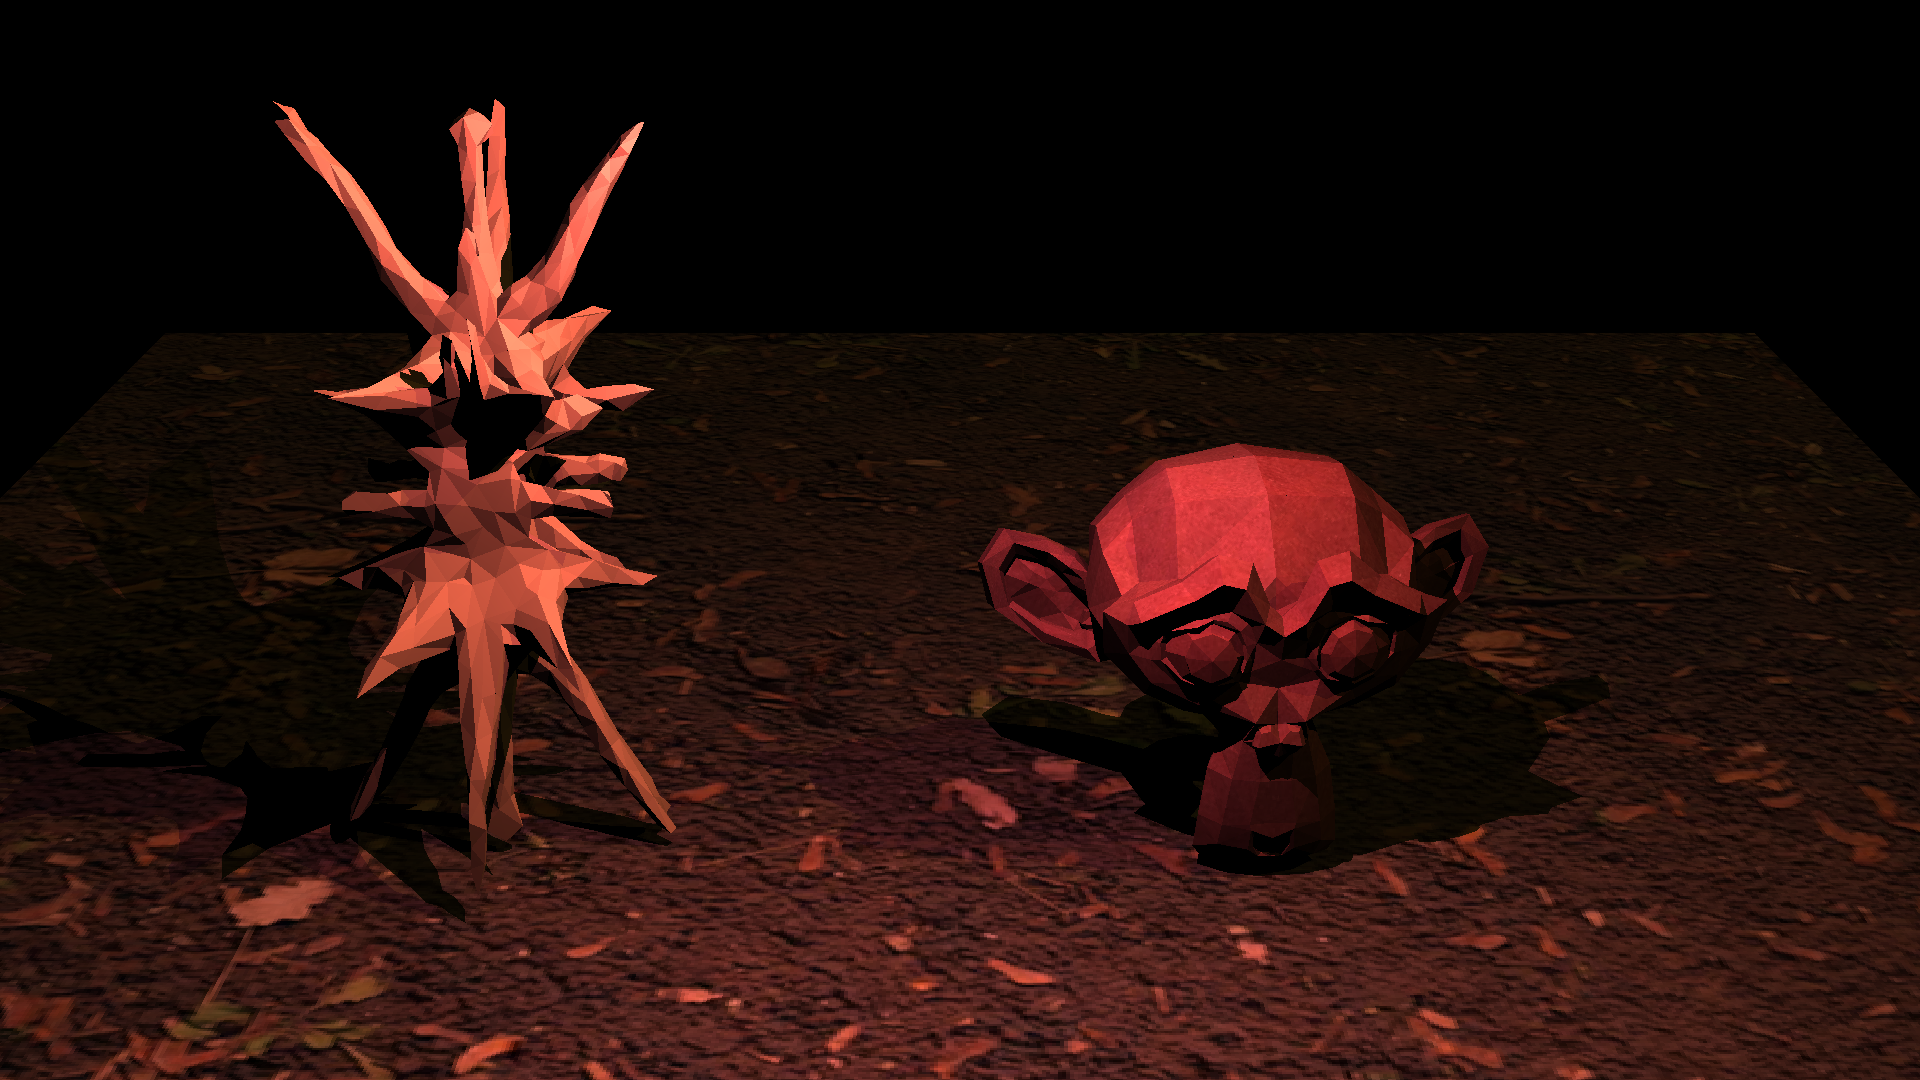
\includegraphics[width=\textwidth]{media/monkey.png}
        \caption{Original Image}
    \end{subfigure}
    \hfill
    \begin{subfigure}[b]{.3\textwidth}
        \centering
        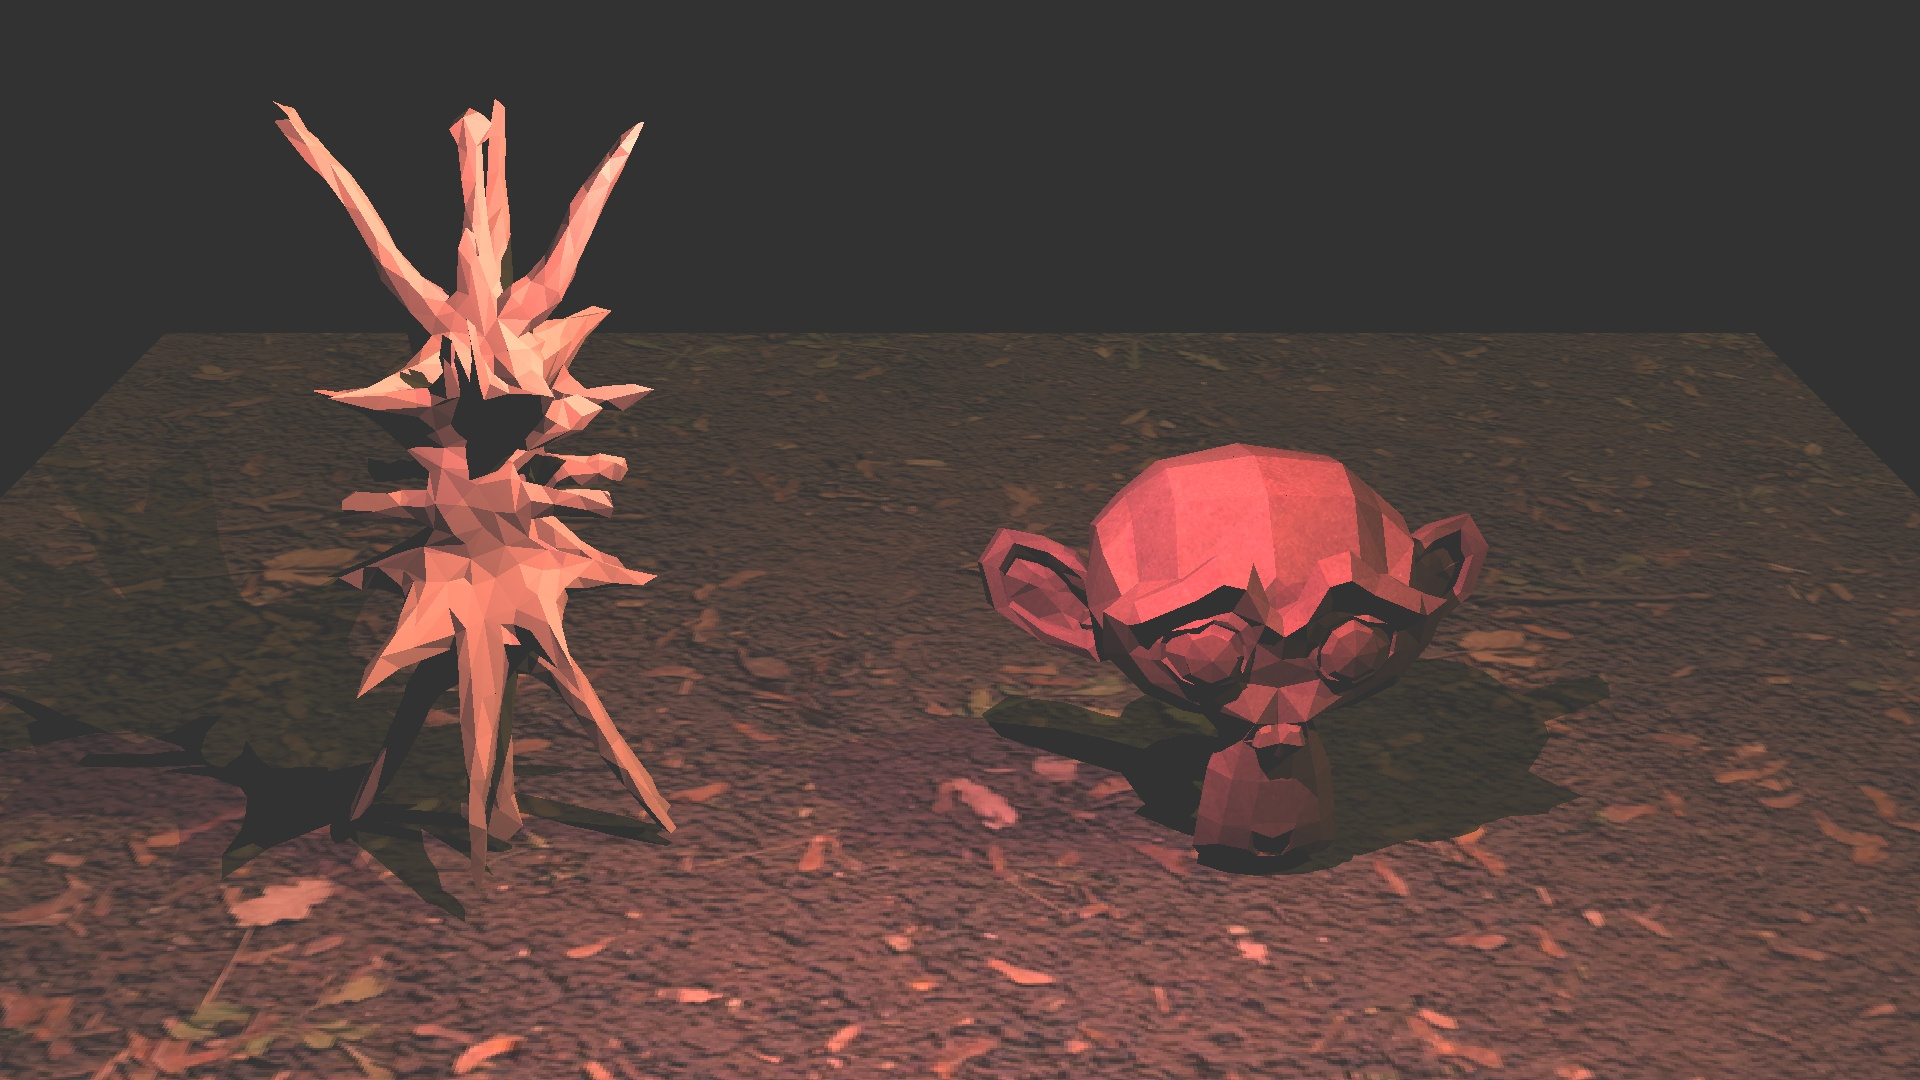
\includegraphics[width=\textwidth]{output/monkey_added_brightness.jpg}
        \caption{Brightness + 50}
    \end{subfigure}
    \hfill
    \begin{subfigure}[b]{.3\textwidth}
        \centering
        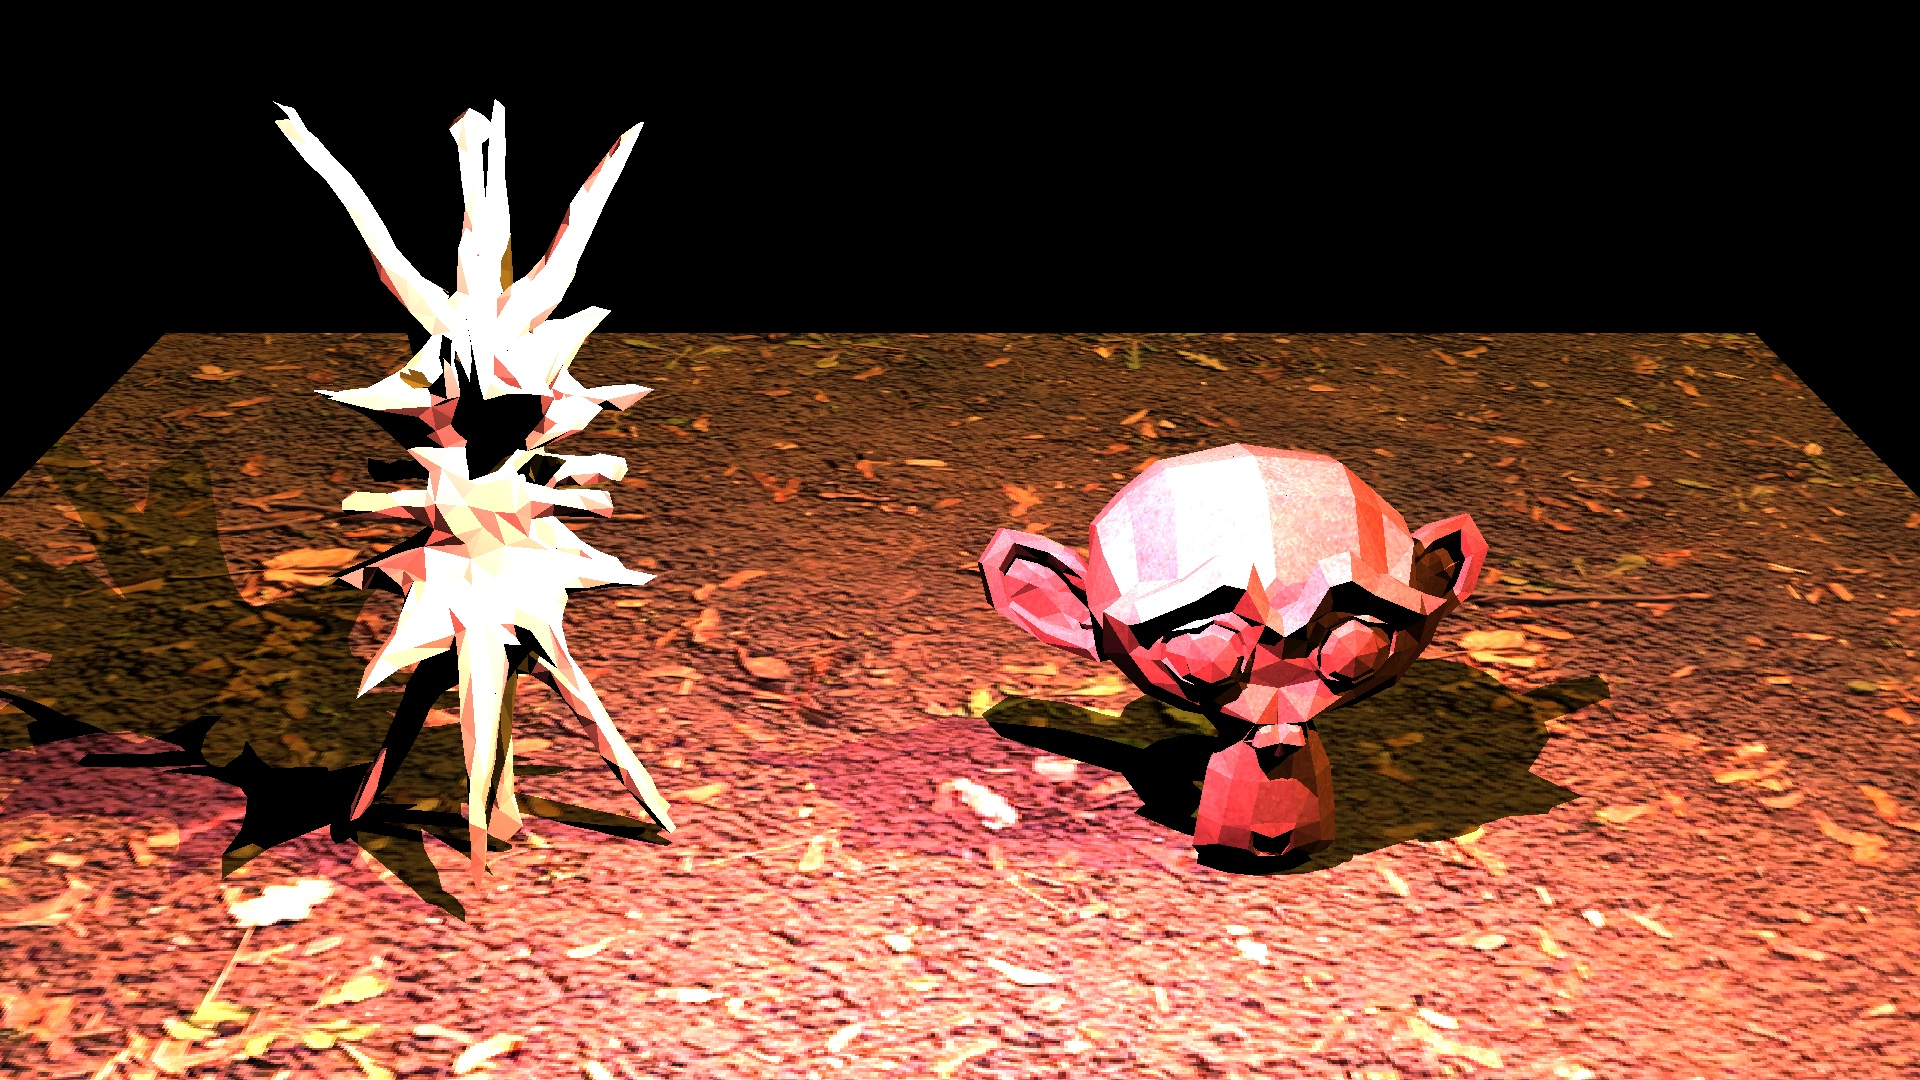
\includegraphics[width=\textwidth]{output/monkey_multiplied_brightness.jpg}
        \caption{Brightness * 5}
    \end{subfigure}
    \hfill
    \caption{Brightness adjustment using modification to intensity values in RGB space.}
    \label{fig:brightness}
\end{figure}

\section{Contrast Stretching}

We now consider an image of trees, covered by fog. We clip the less frequent intensity values and remap the remaining to the entire color space. This transformation reveals not just the trees, but also the discontinuities present in the snow.

\begin{figure}[H]
    \hfill
    \centering
    \begin{subfigure}[b]{.225\textwidth}
        \centering
        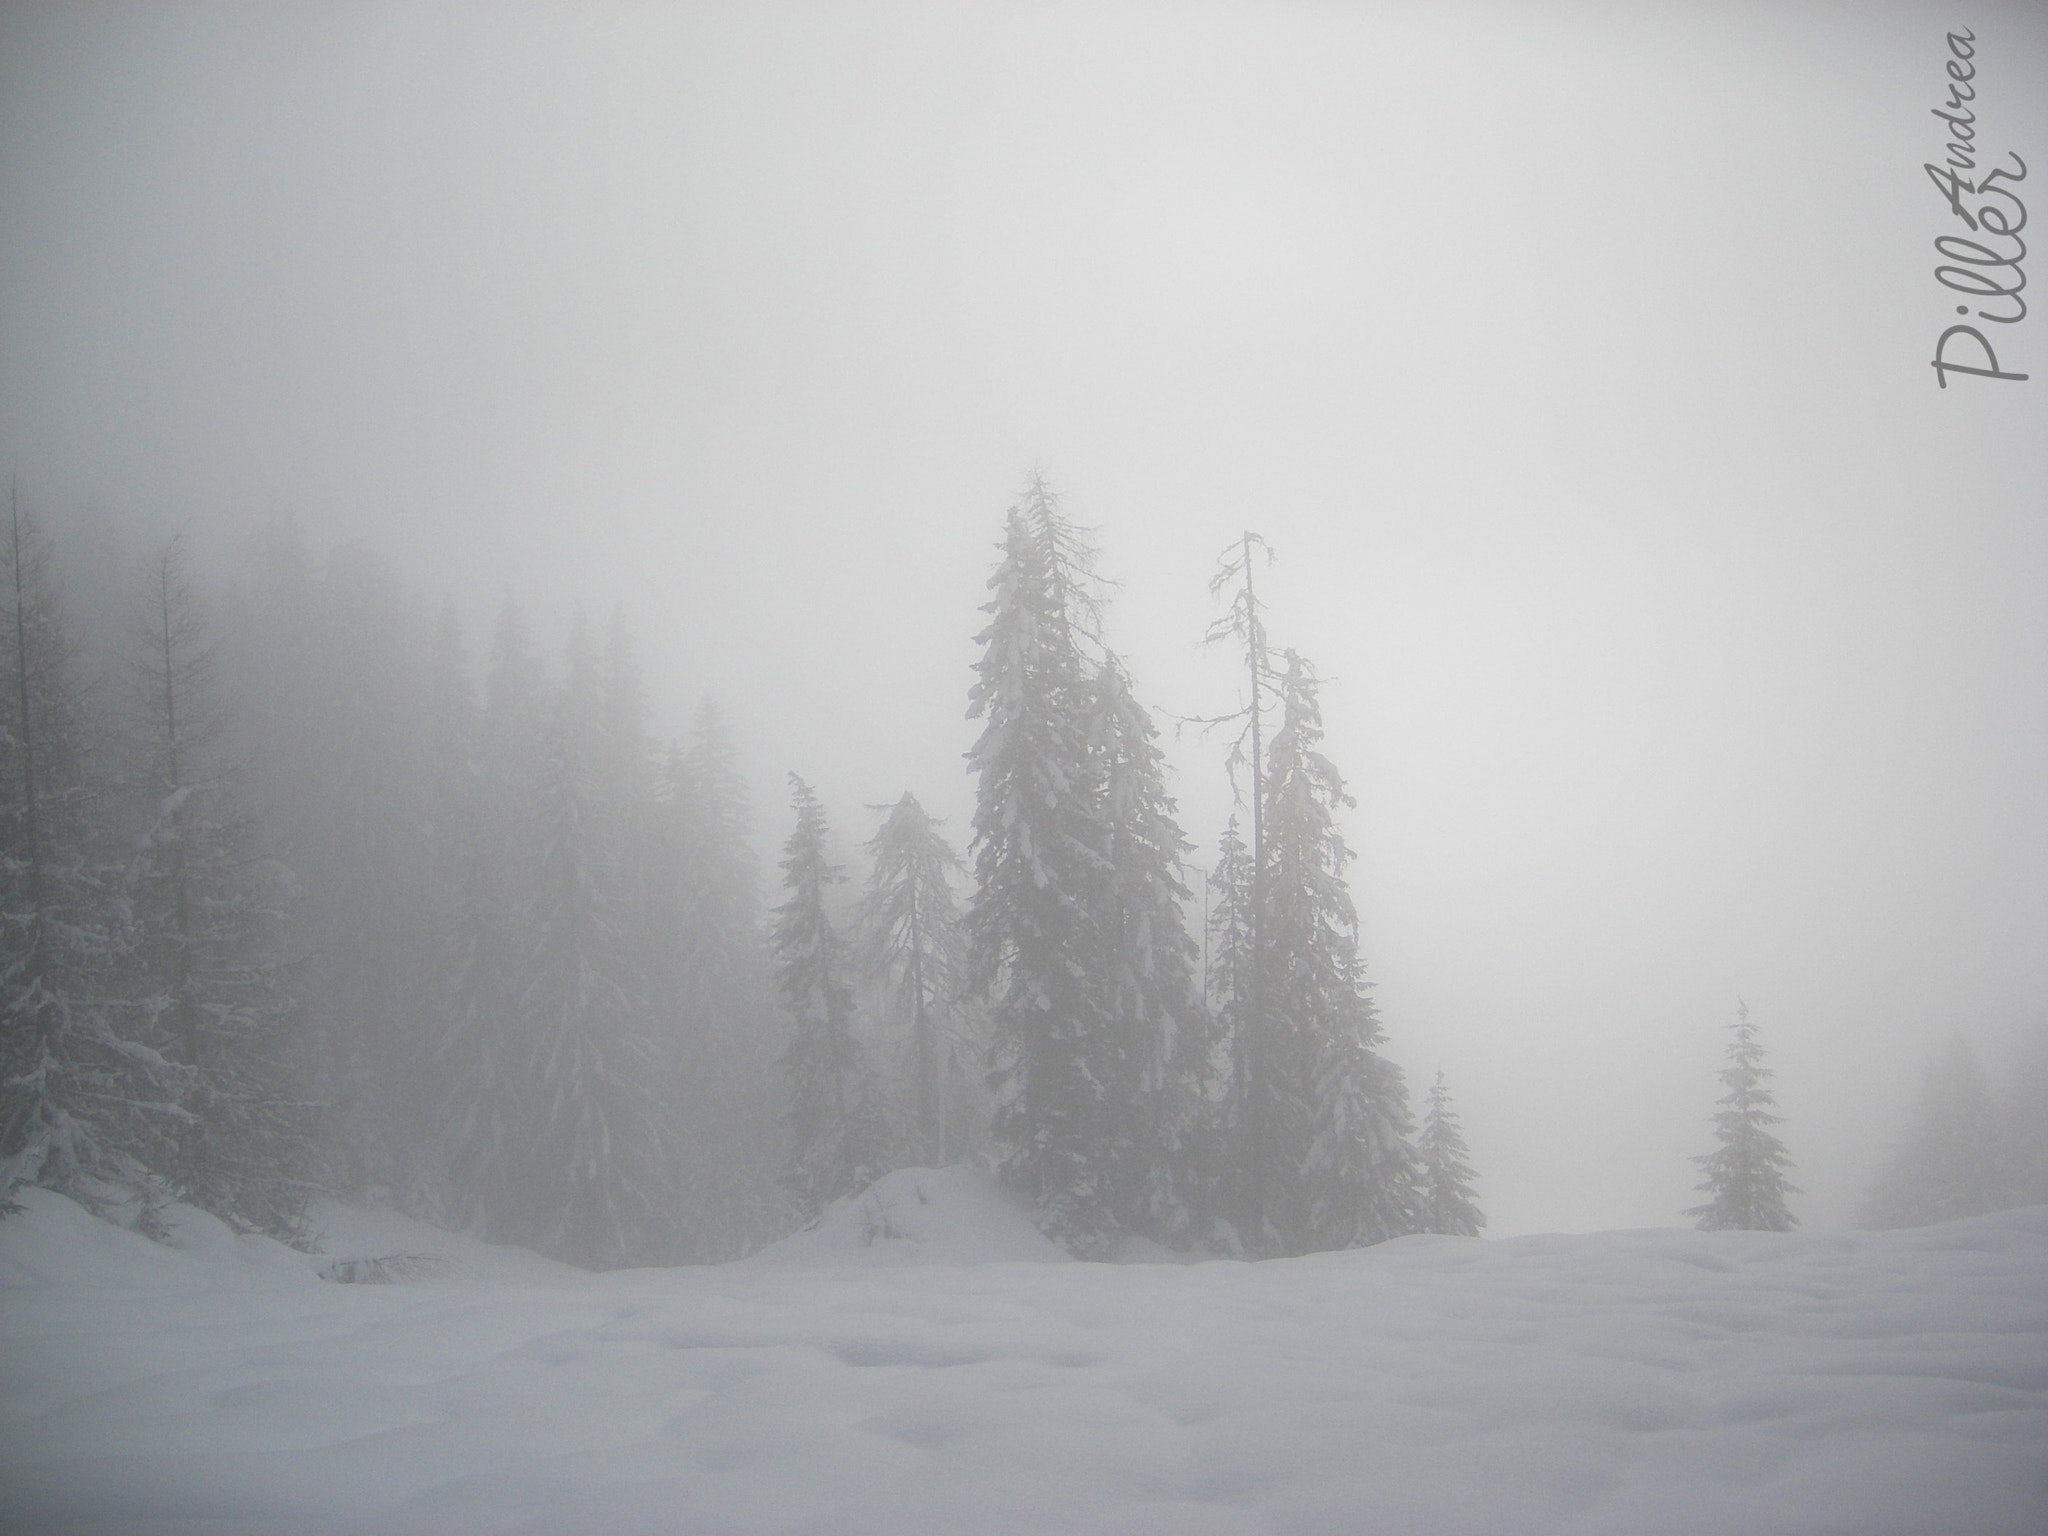
\includegraphics[width=\textwidth]{media/fog.jpg}
        \caption{Original Image}
    \end{subfigure}
    \hfill
    \begin{subfigure}[b]{.225\textwidth}
        \centering
        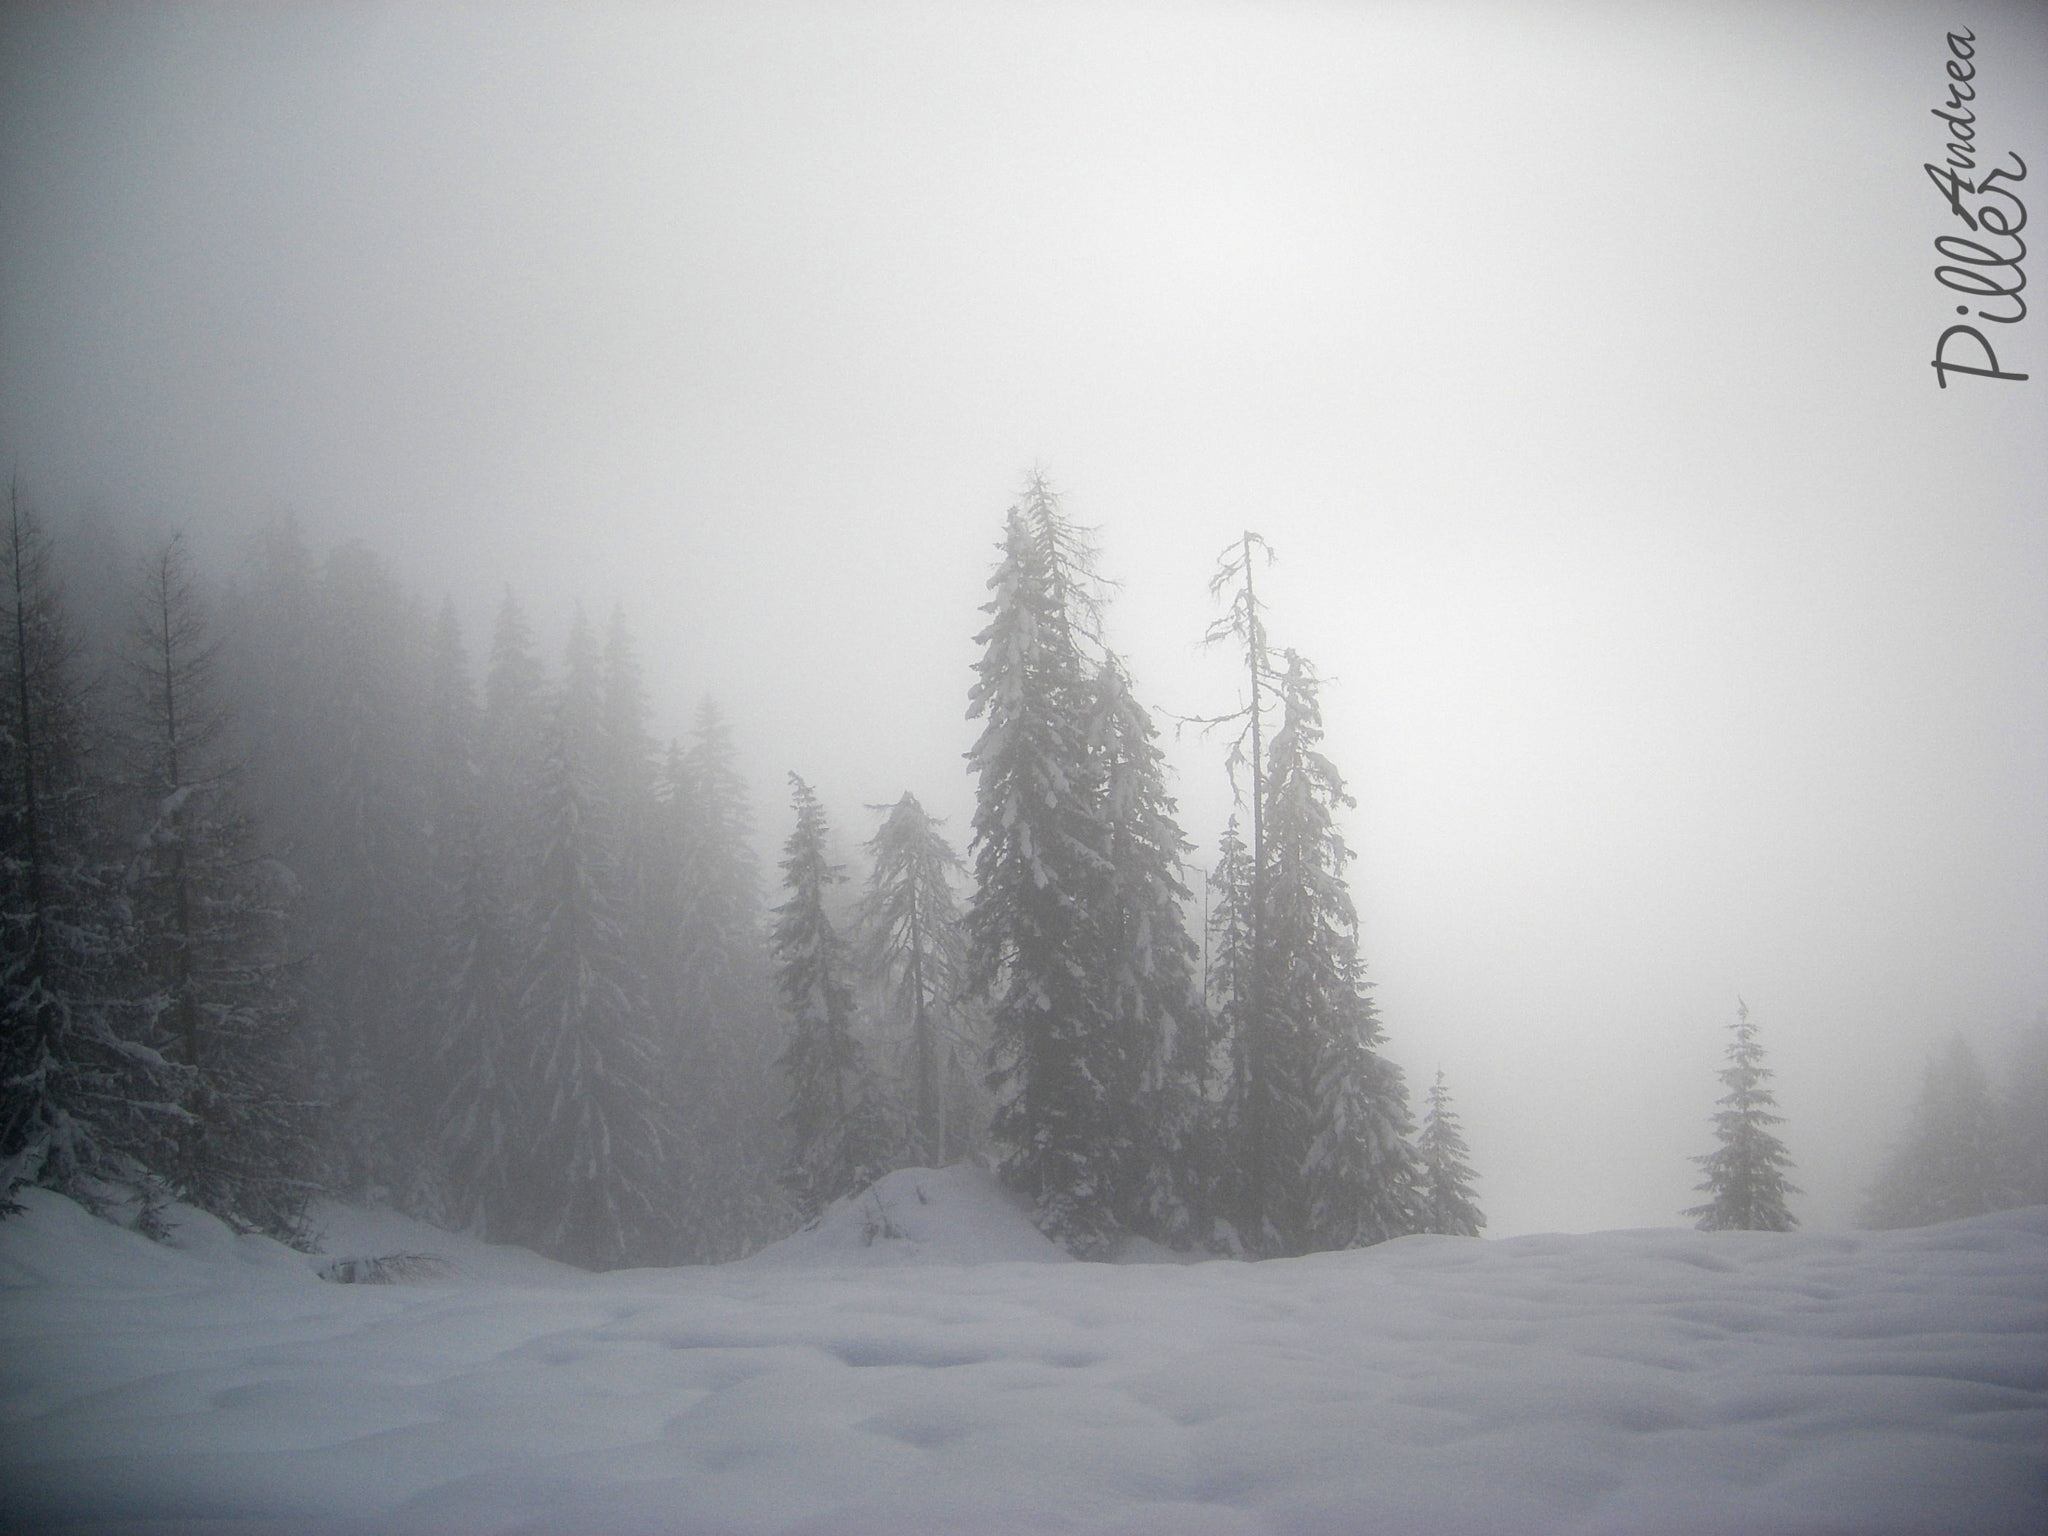
\includegraphics[width=\textwidth]{output/fog_contrast.jpg}
        \caption{Min Max Clipping}
    \end{subfigure}
    \hfill
    \begin{subfigure}[b]{.225\textwidth}
        \centering
        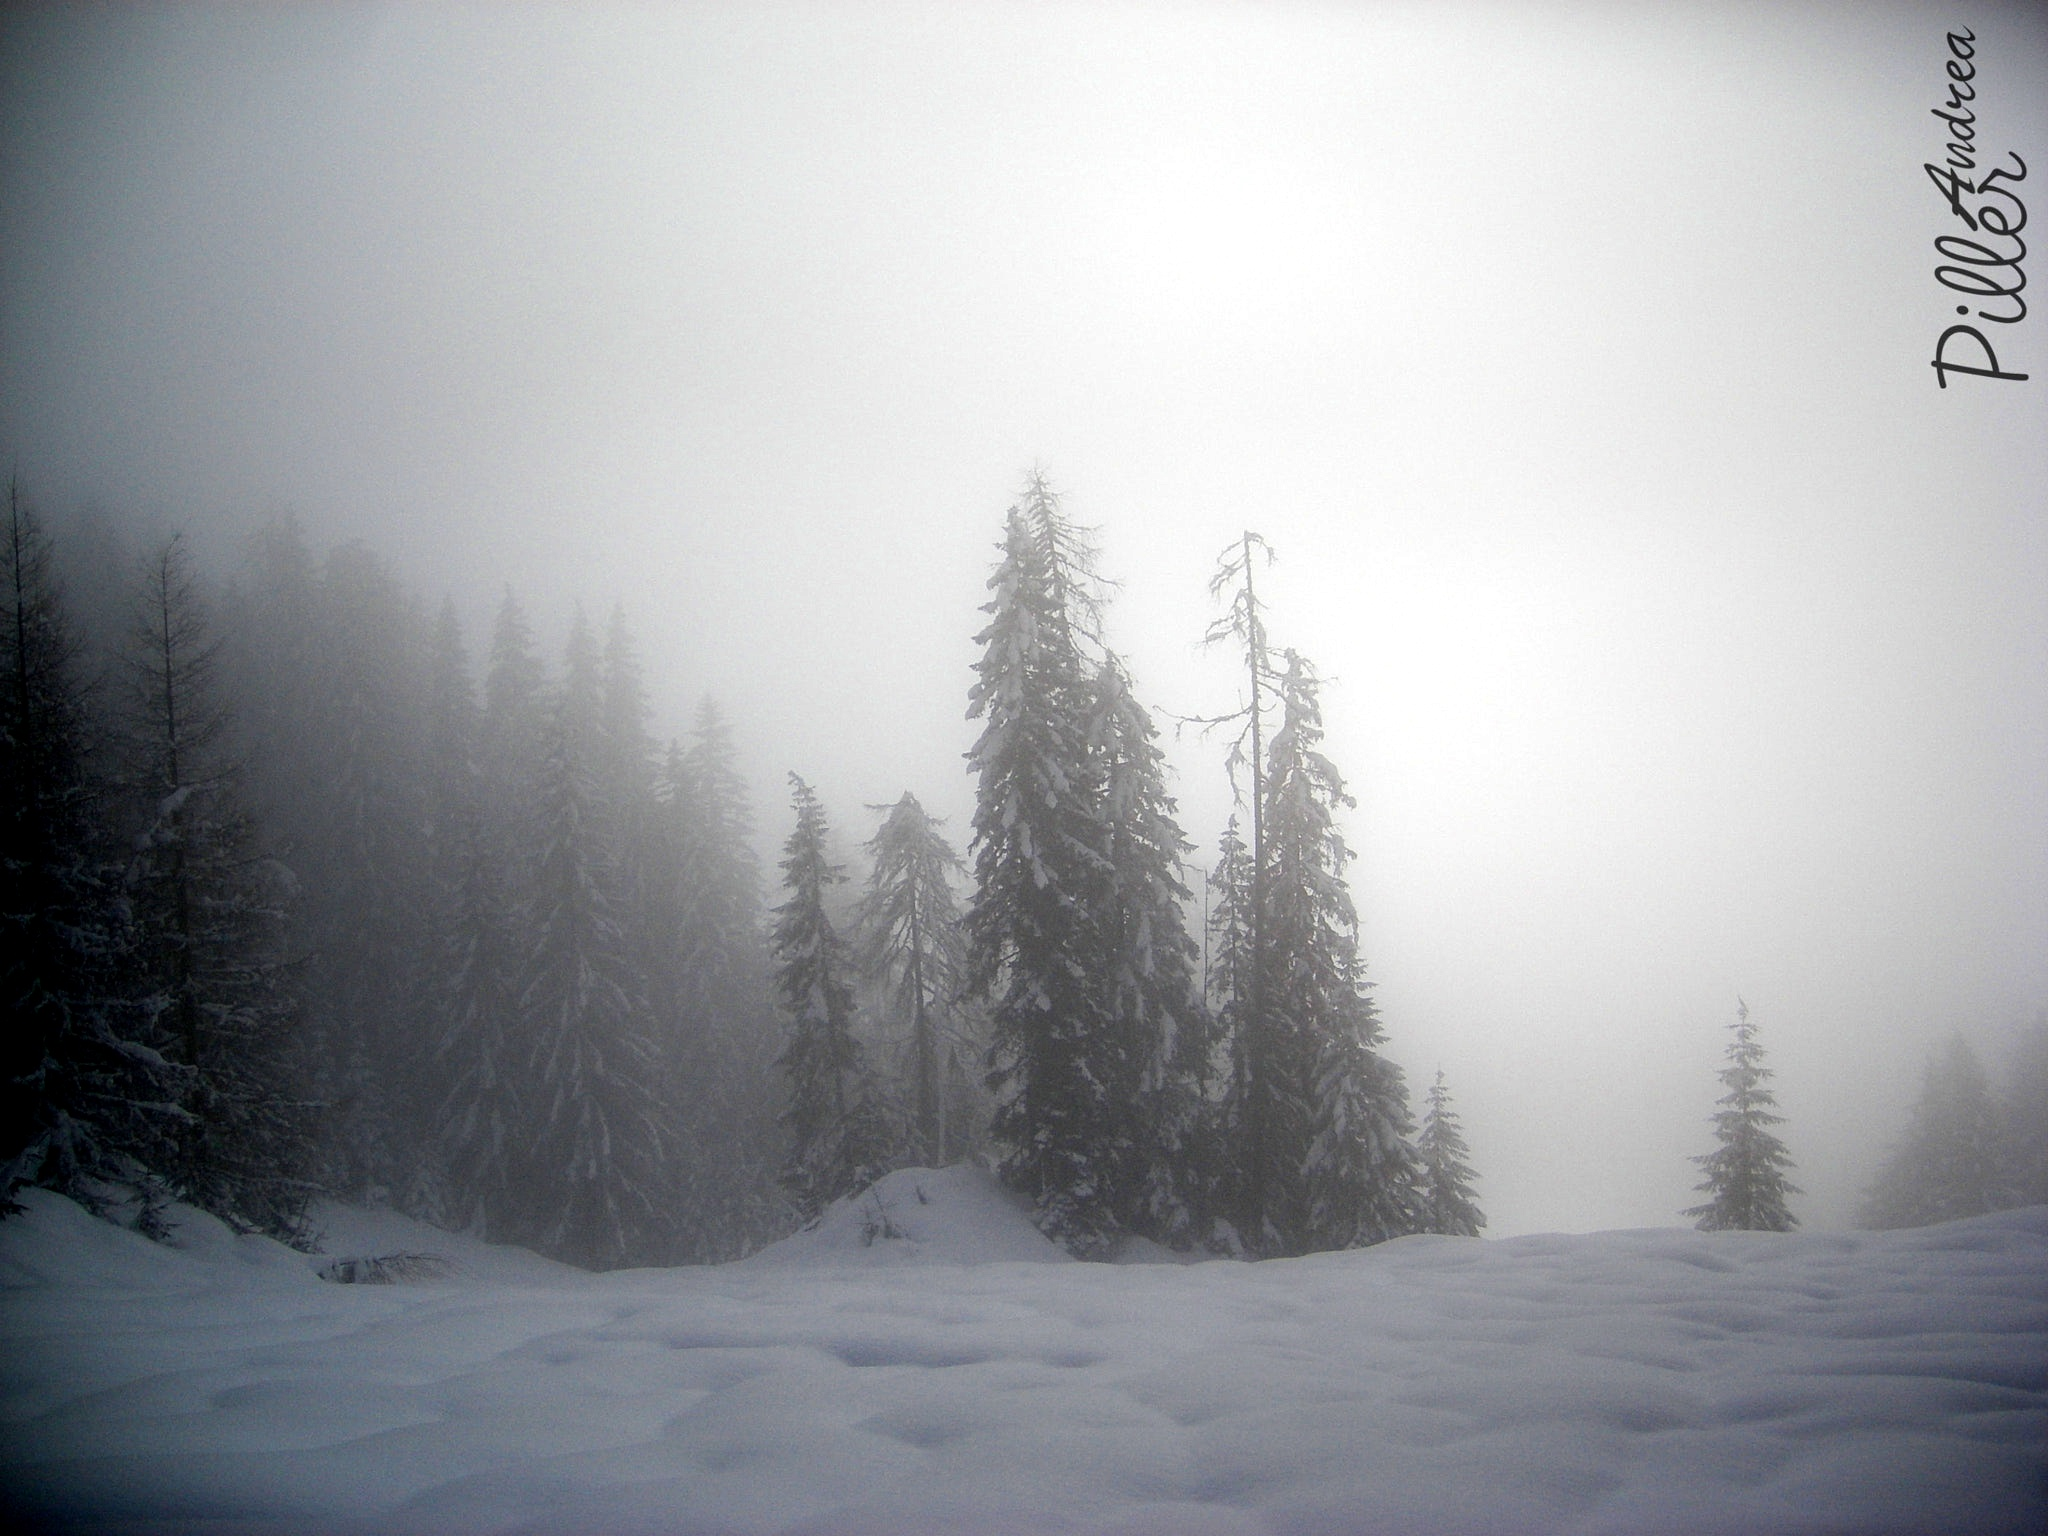
\includegraphics[width=\textwidth]{output/fog_contrast_1.jpg}
        \caption{1 Percentile}
    \end{subfigure}
    \hfill
    \begin{subfigure}[b]{.225\textwidth}
        \centering
        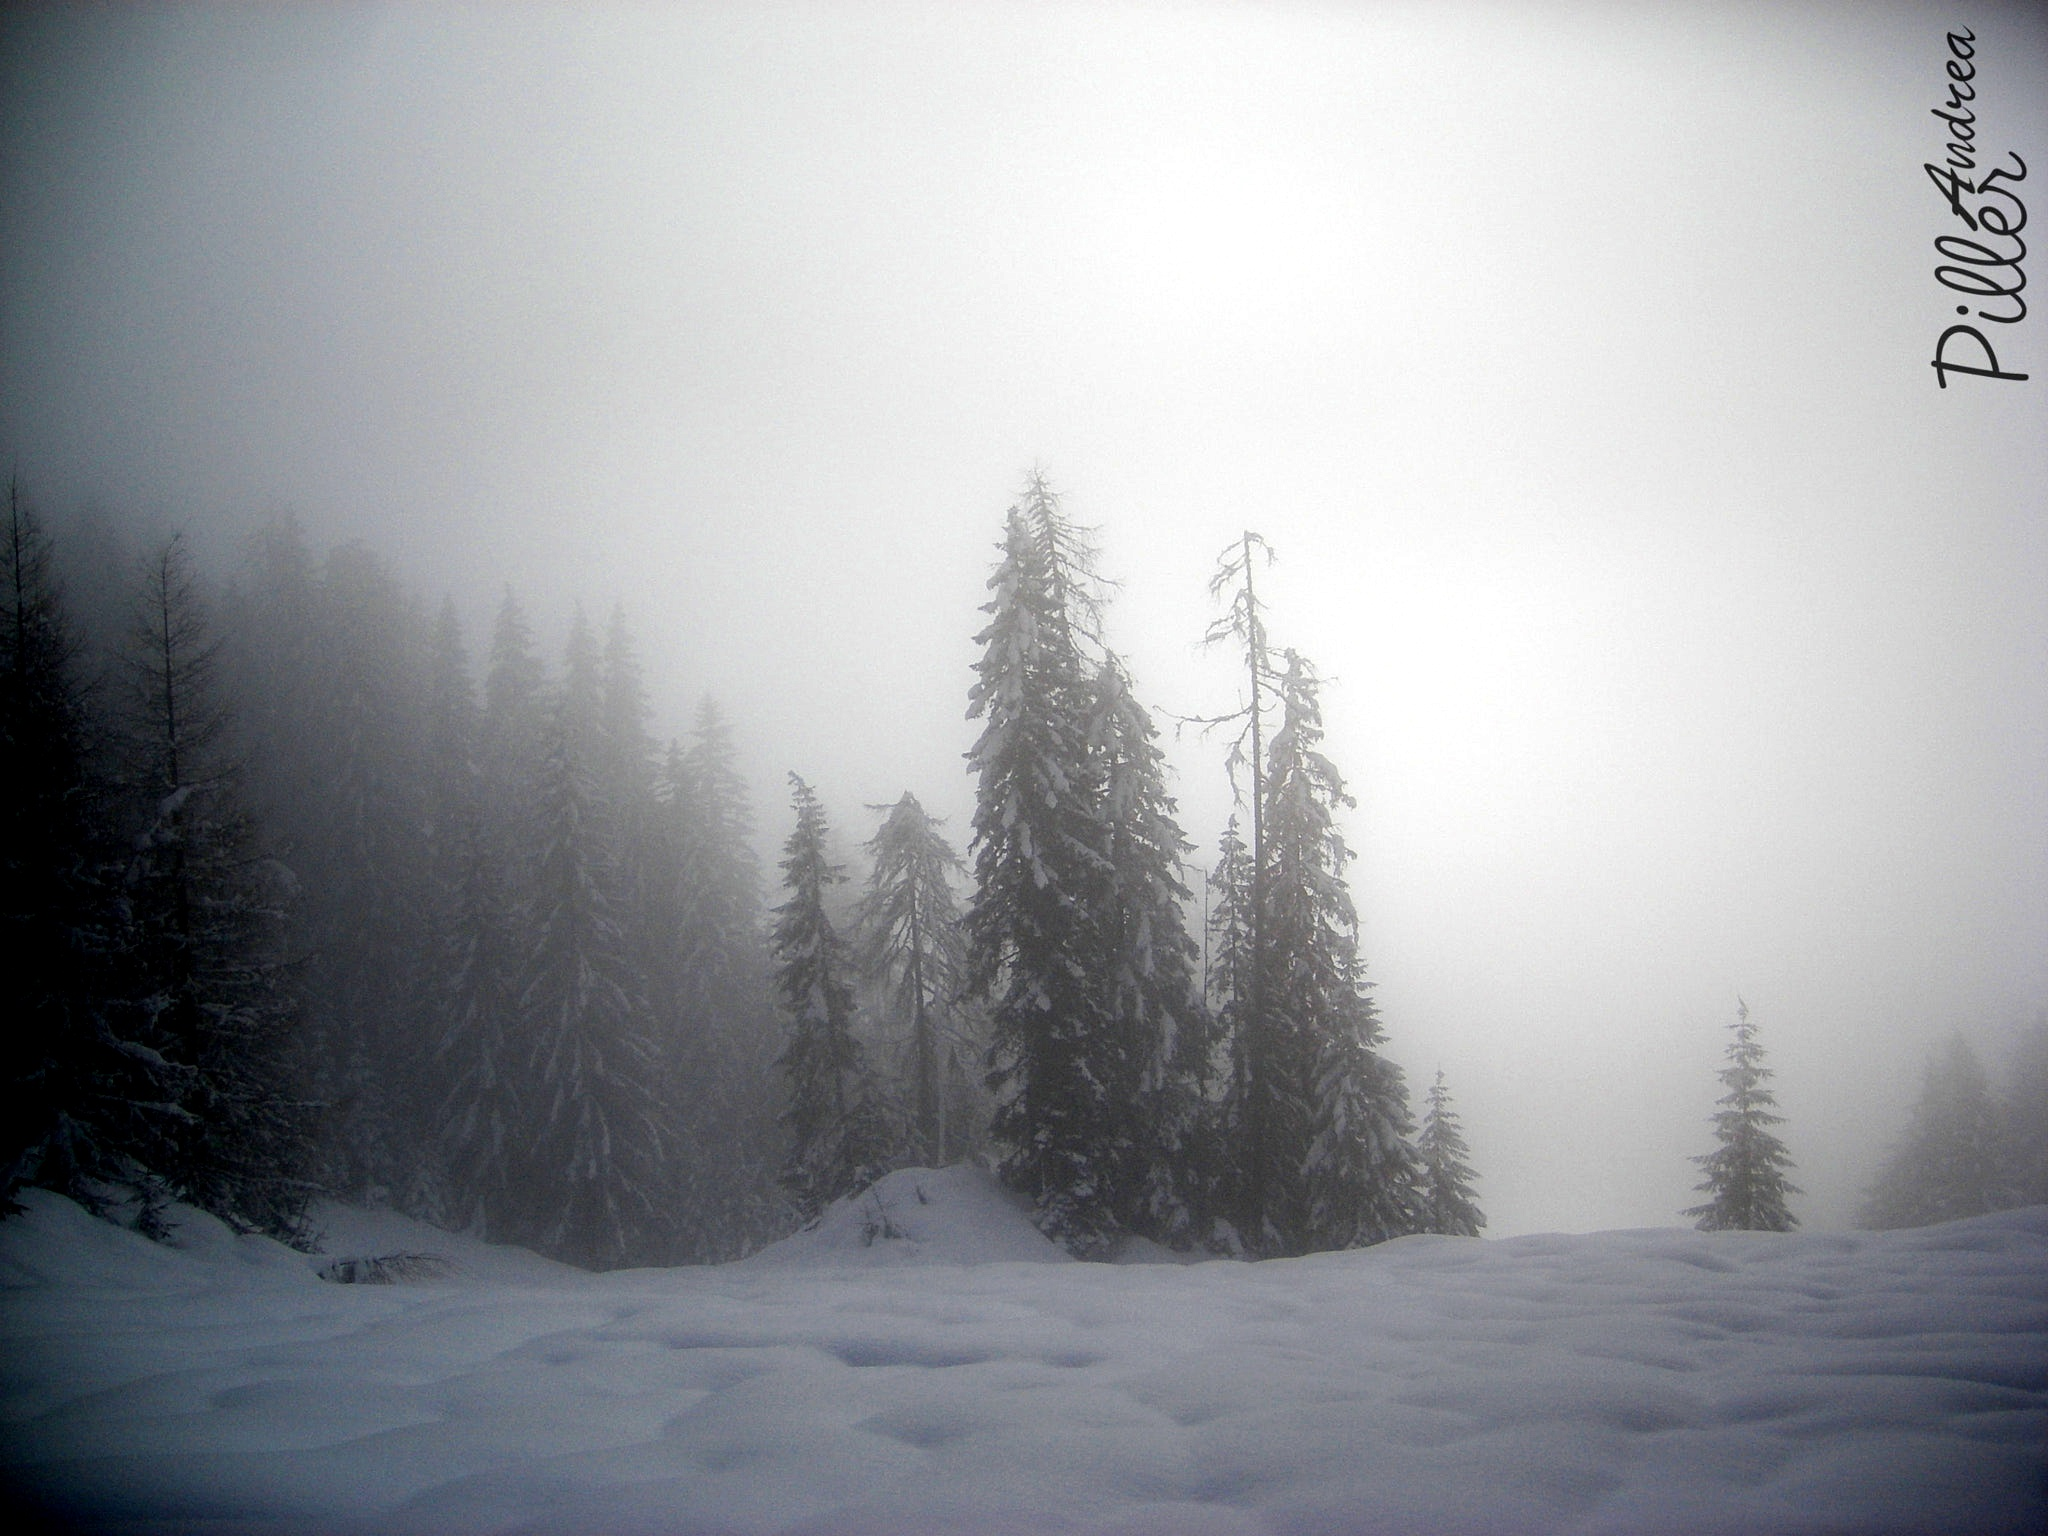
\includegraphics[width=\textwidth]{output/fog_contrast_2.jpg}
        \caption{2 Percentile}
    \end{subfigure}
    \hfill
    \caption{Contrast stretching by thresholding intensity values at various levels.}
    \label{fig:contrast}
\end{figure}

\section{Grayscale Conversion}

We move on to consider an image of a pink rose. The image consists of both light and dark shades of pink. The former consisting of almost equal proportion of blue intensity values to red. We use weighted average, weights set according to uniform distribution, ITU BT.601 and BT.709. Surprisingly, the details of the rose become more prominent, even though we decrease the weight assigned to red channel (presumably due to the way humans perceive colors).

\begin{figure}[H]
    \hfill
    \centering
    \begin{subfigure}[b]{.225\textwidth}
        \centering
        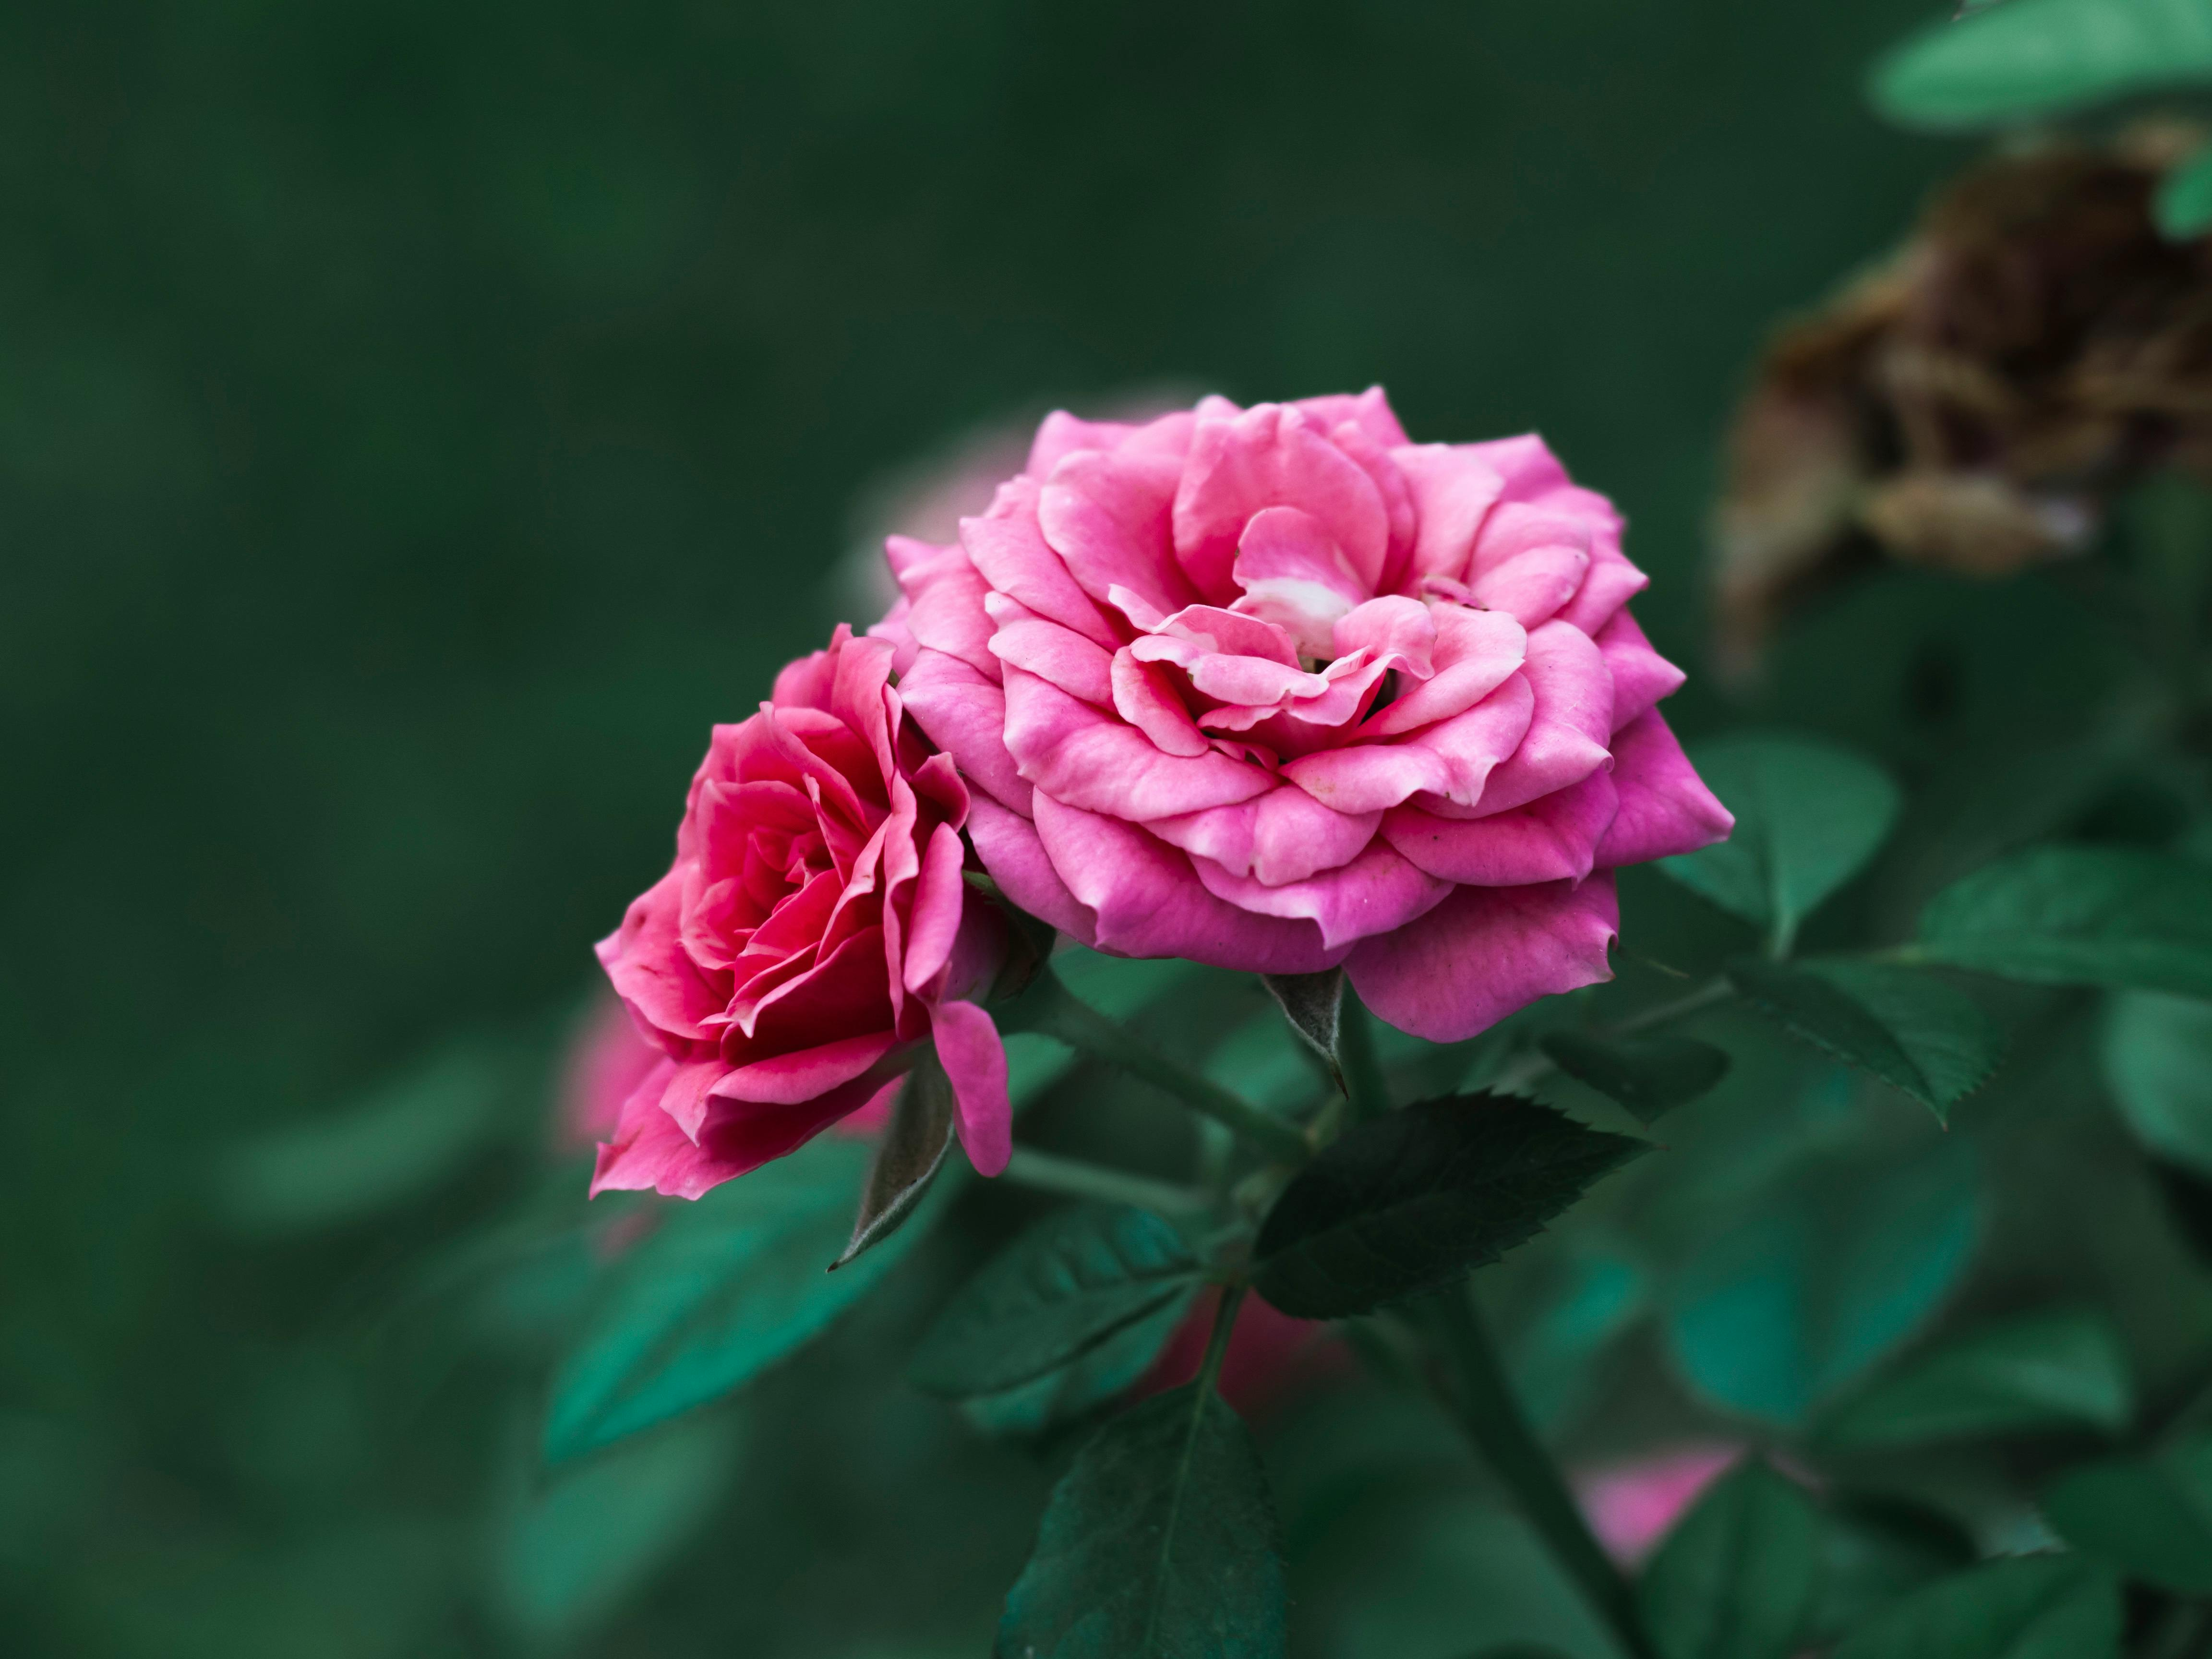
\includegraphics[width=\textwidth]{media/rose.jpg}
        \caption{Original Image}
    \end{subfigure}
    \hfill
    \begin{subfigure}[b]{.225\textwidth}
        \centering
        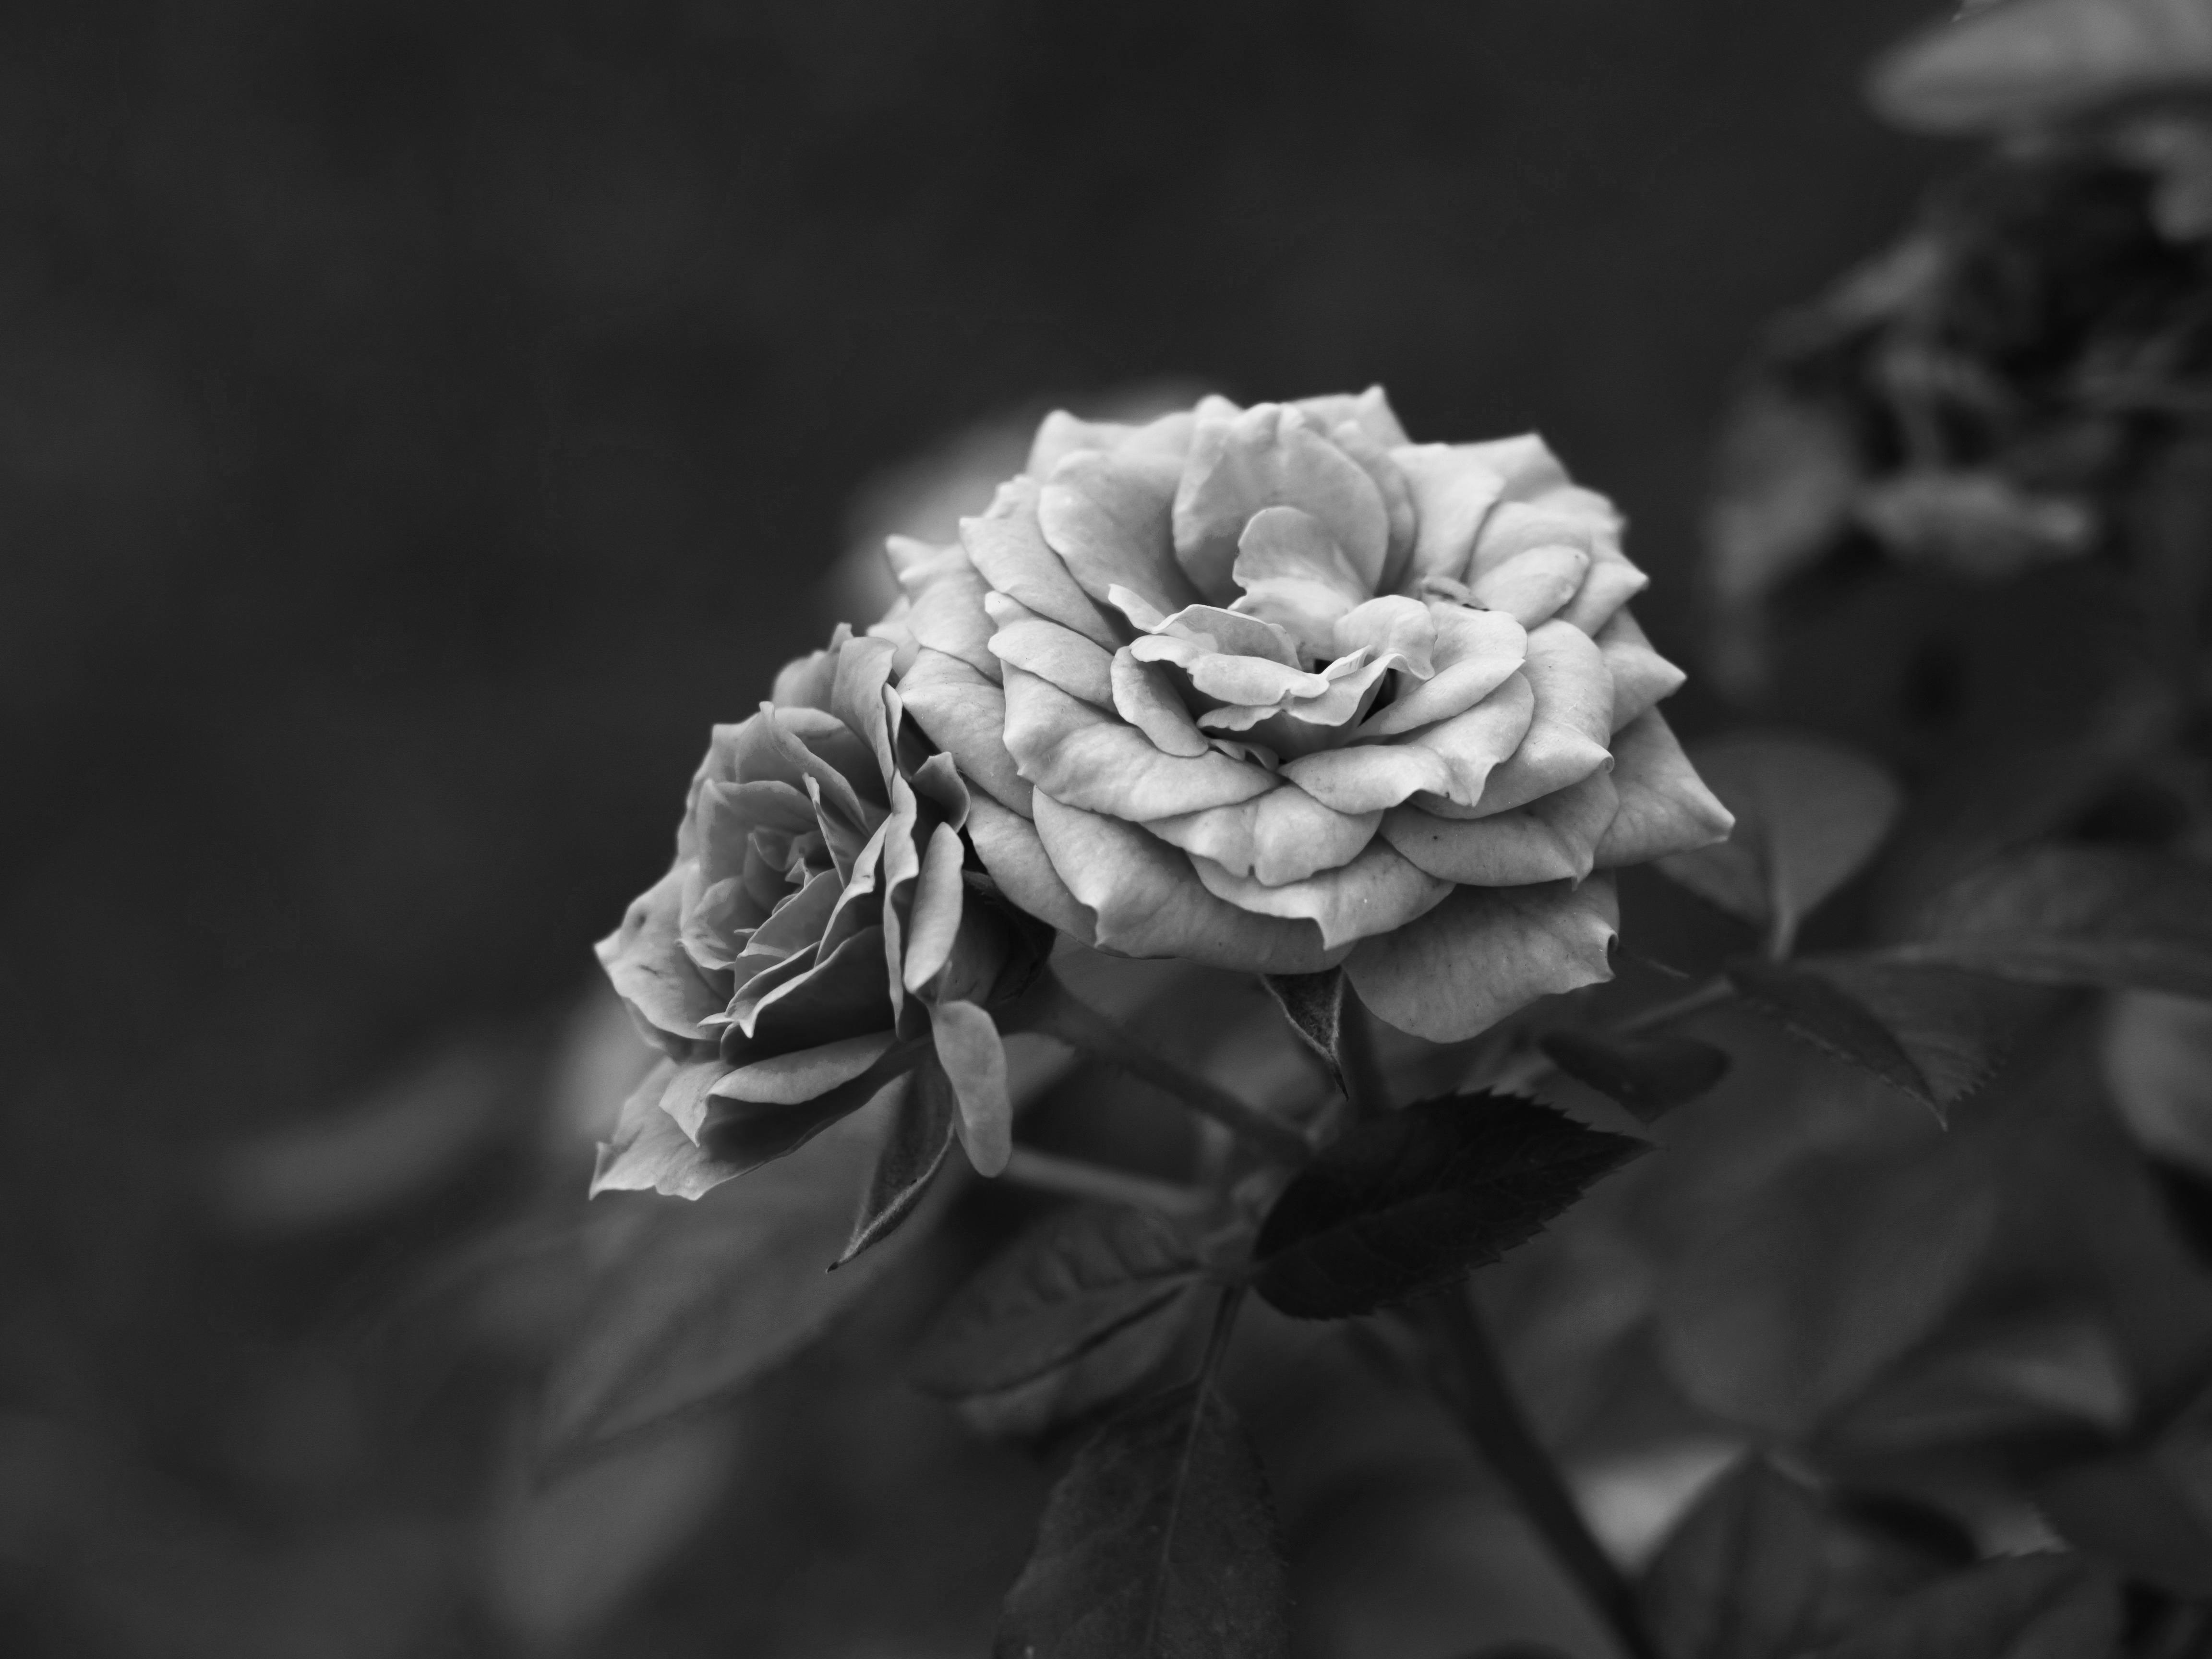
\includegraphics[width=\textwidth]{output/rose_grayscale_33.jpg}
        \caption{33\%}
    \end{subfigure}
    \hfill
    \begin{subfigure}[b]{.225\textwidth}
        \centering
        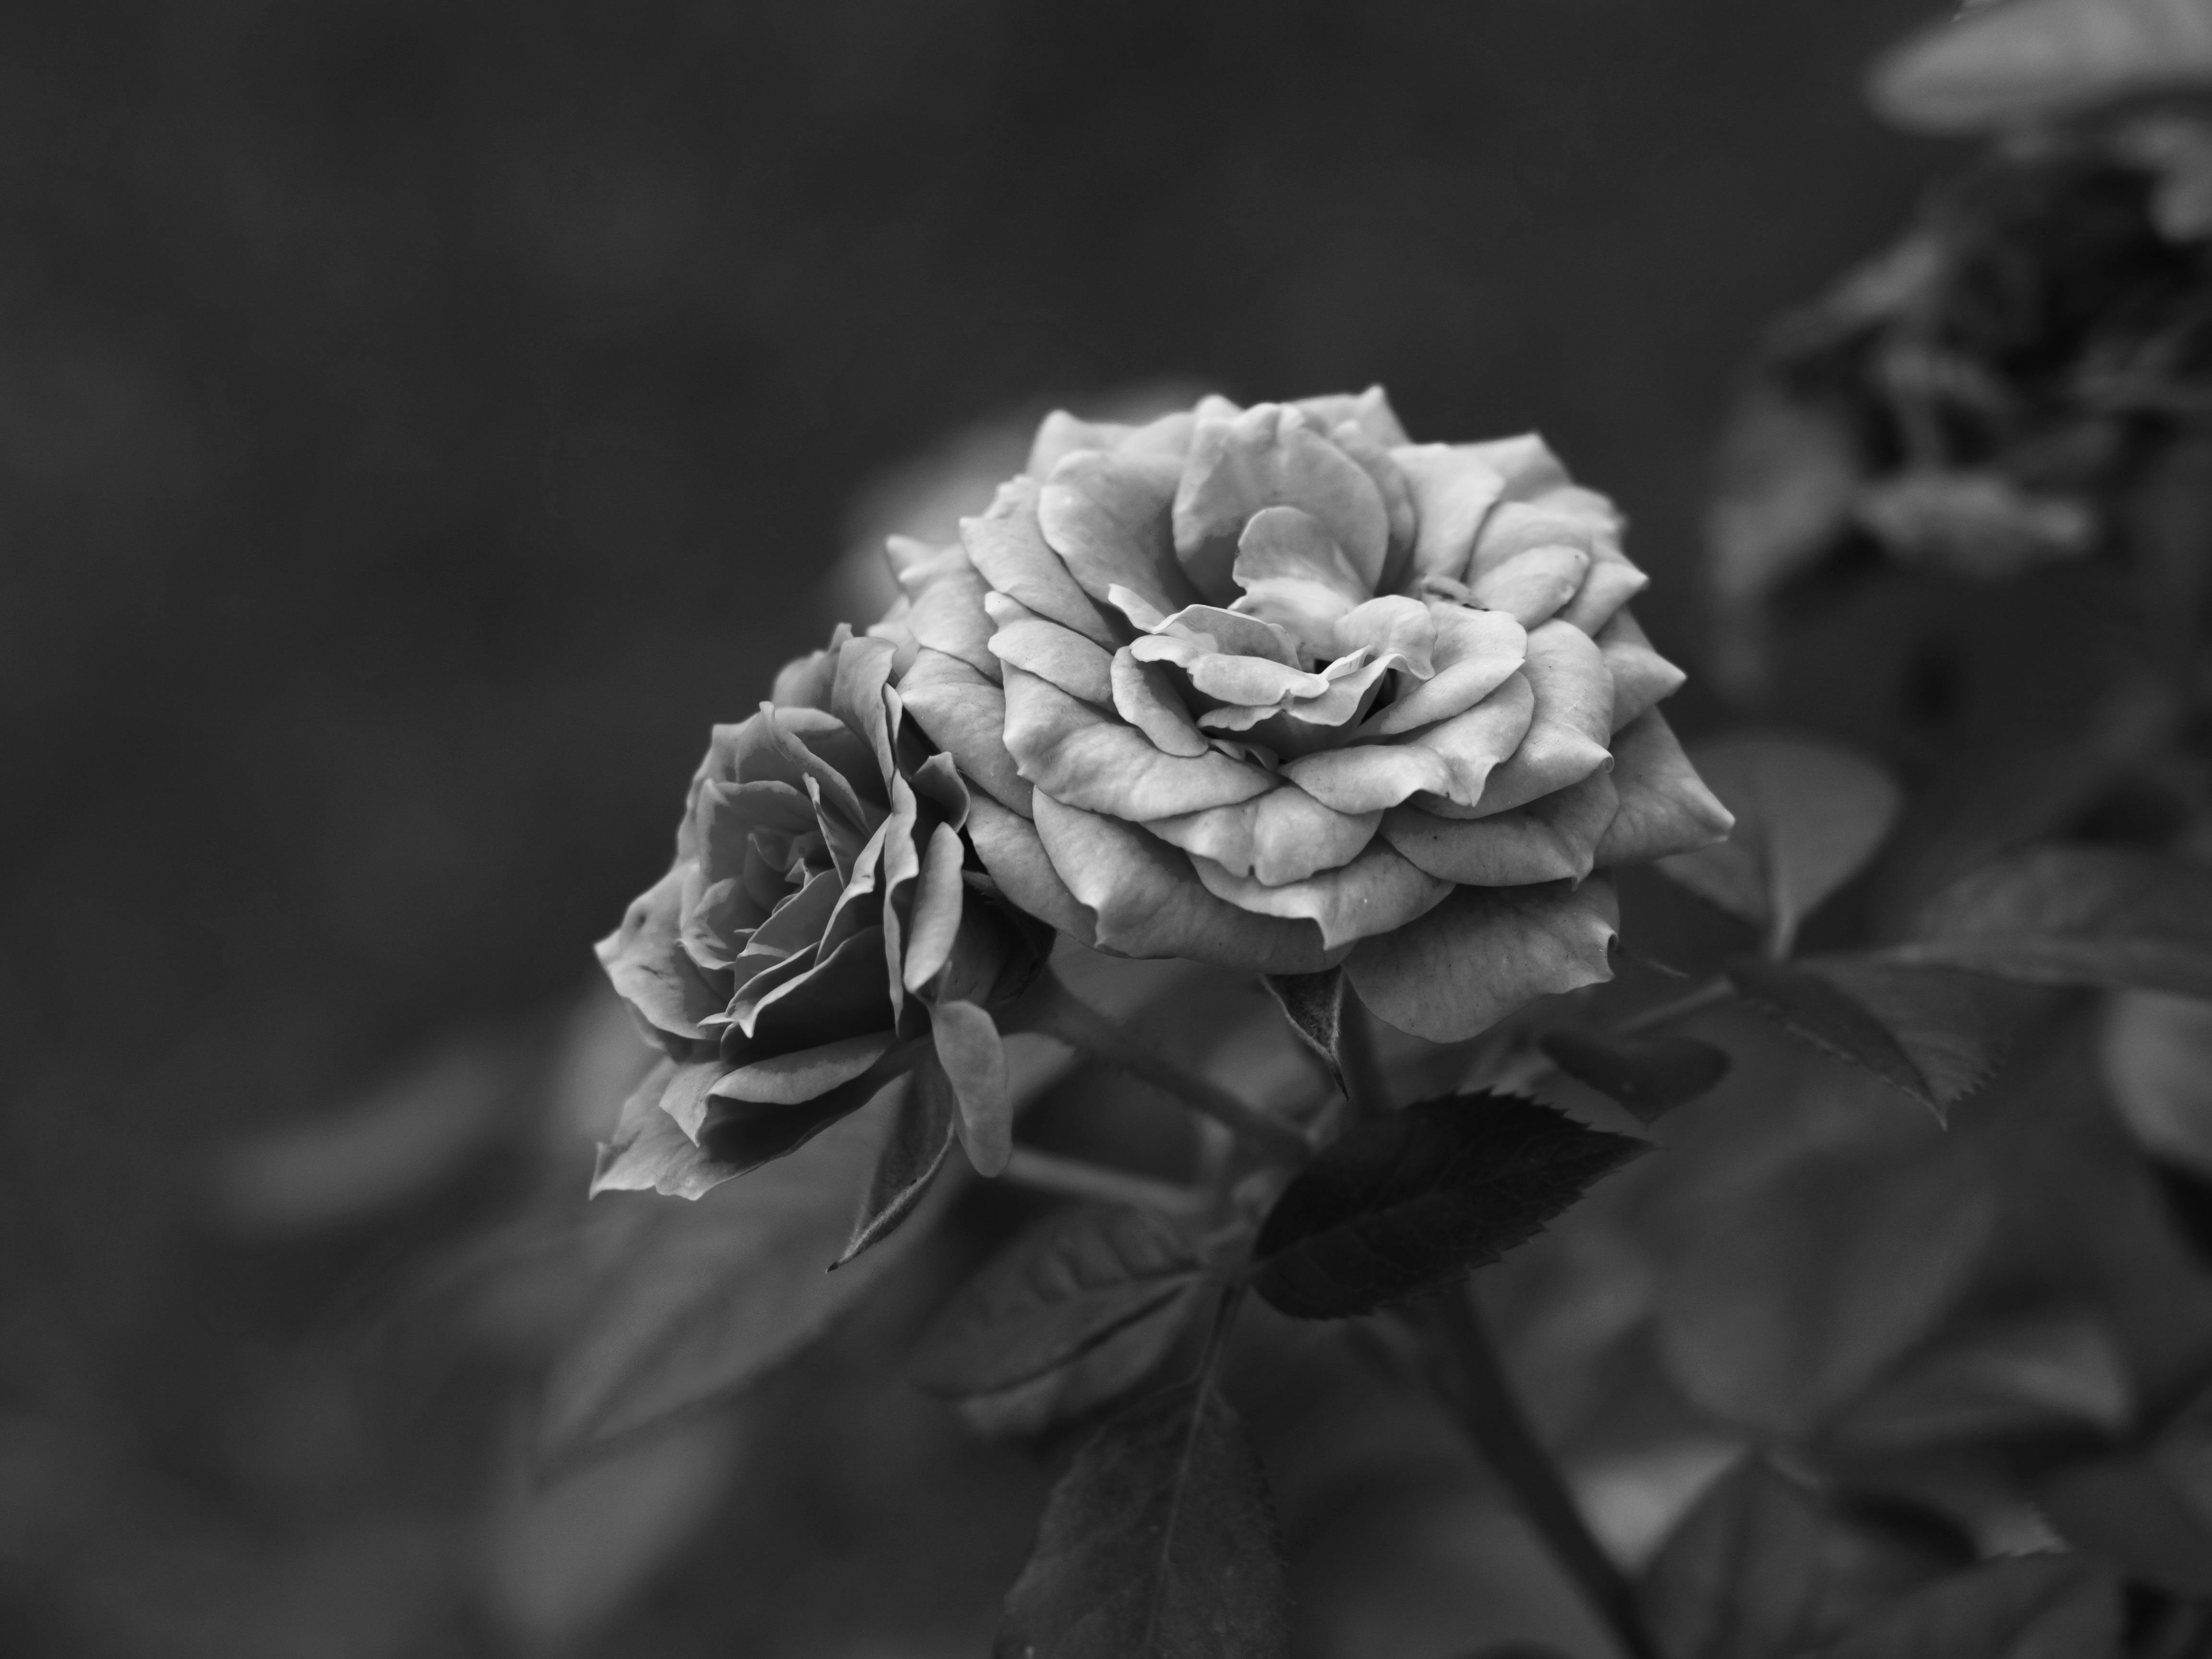
\includegraphics[width=\textwidth]{output/rose_grayscale_60.jpg}
        \caption{60\%}
    \end{subfigure}
    \hfill
    \begin{subfigure}[b]{.225\textwidth}
        \centering
        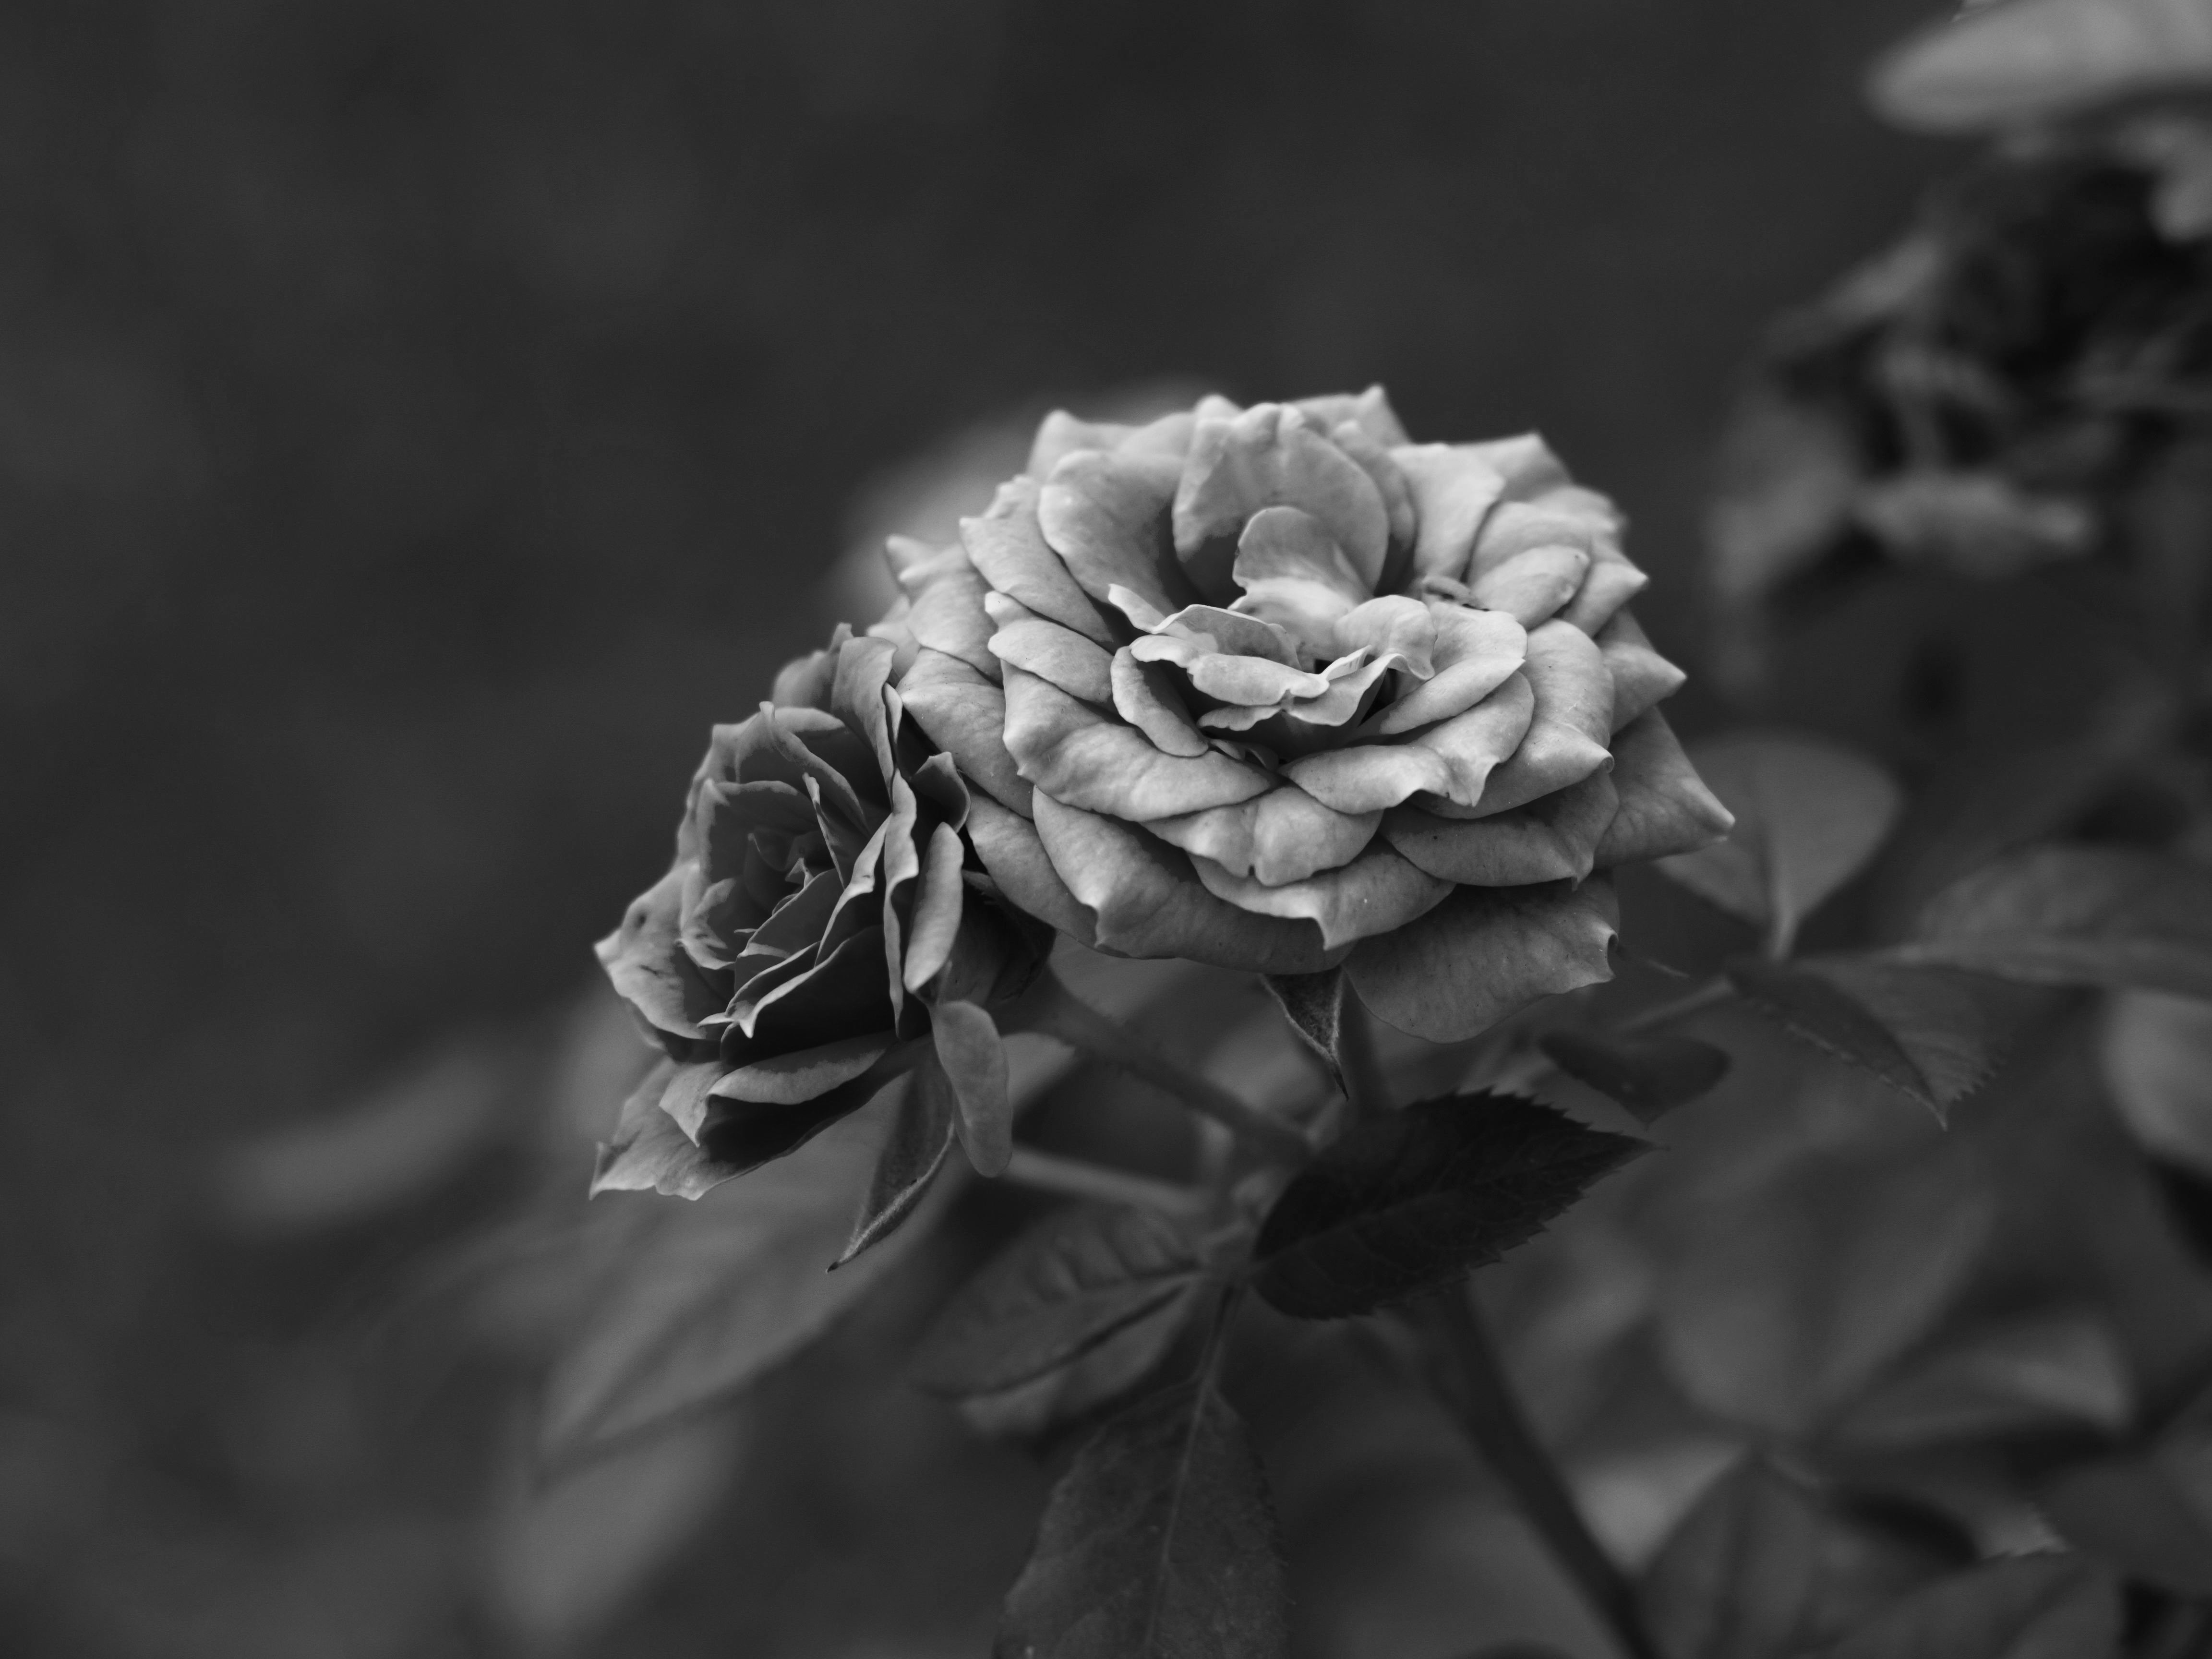
\includegraphics[width=\textwidth]{output/rose_grayscale_70.jpg}
        \caption{70\%}
    \end{subfigure}
    \hfill
    \caption{Conversion to grayscale using weighted avergae, with different weights assigned to green channel.}
    \label{fig:grayscale}
\end{figure}

\section{Pseudo Color Mapping}

For pseduo coloring, we use an image of a peacock feather, with separately visible red, green and blue regions. We use a simple gradient map on the grayscale image, that varies from green in the top left corner to saffron in the bottom right. The resulting output happens to be a close match to the original image. Perhaps, incorporating blue in the top right corner for the gradient, would have made this more conclusive.

\begin{figure}[H]
    \hfill
    \centering
    \begin{subfigure}[b]{.225\textwidth}
        \centering
        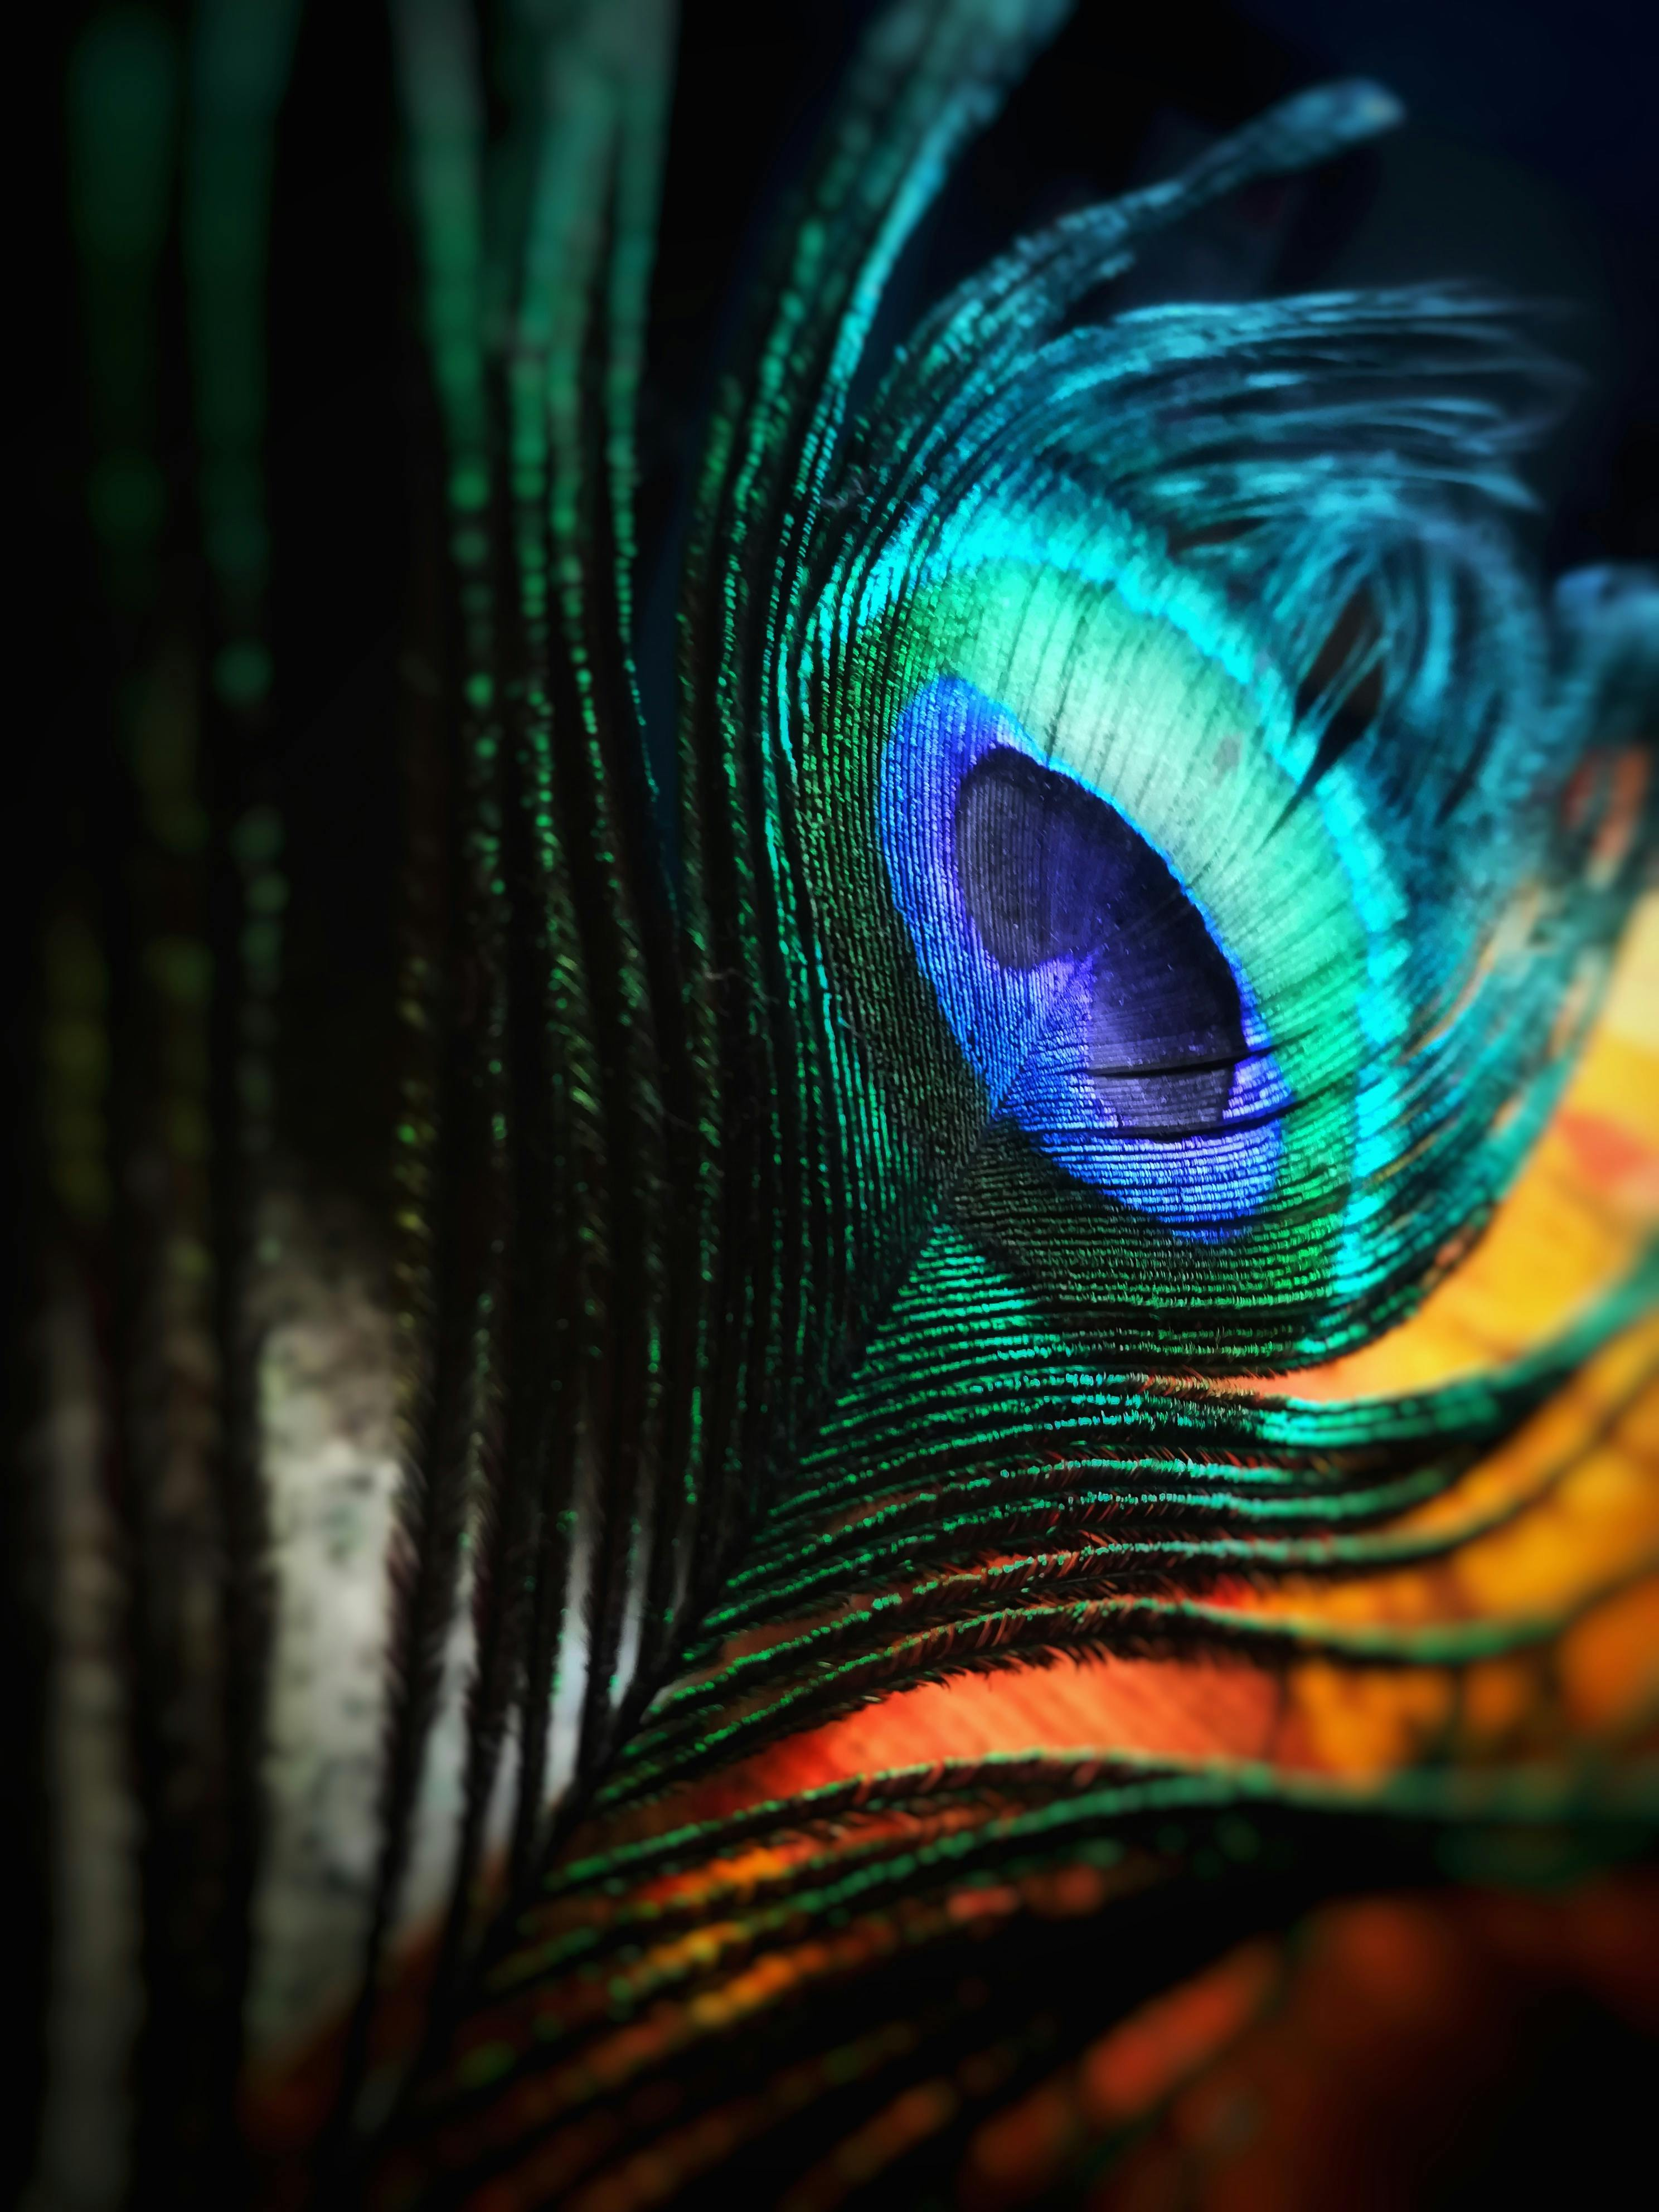
\includegraphics[width=\textwidth]{media/feather.jpg}
        \caption{Original Image}
    \end{subfigure}
    \hfill
    \begin{subfigure}[b]{.225\textwidth}
        \centering
        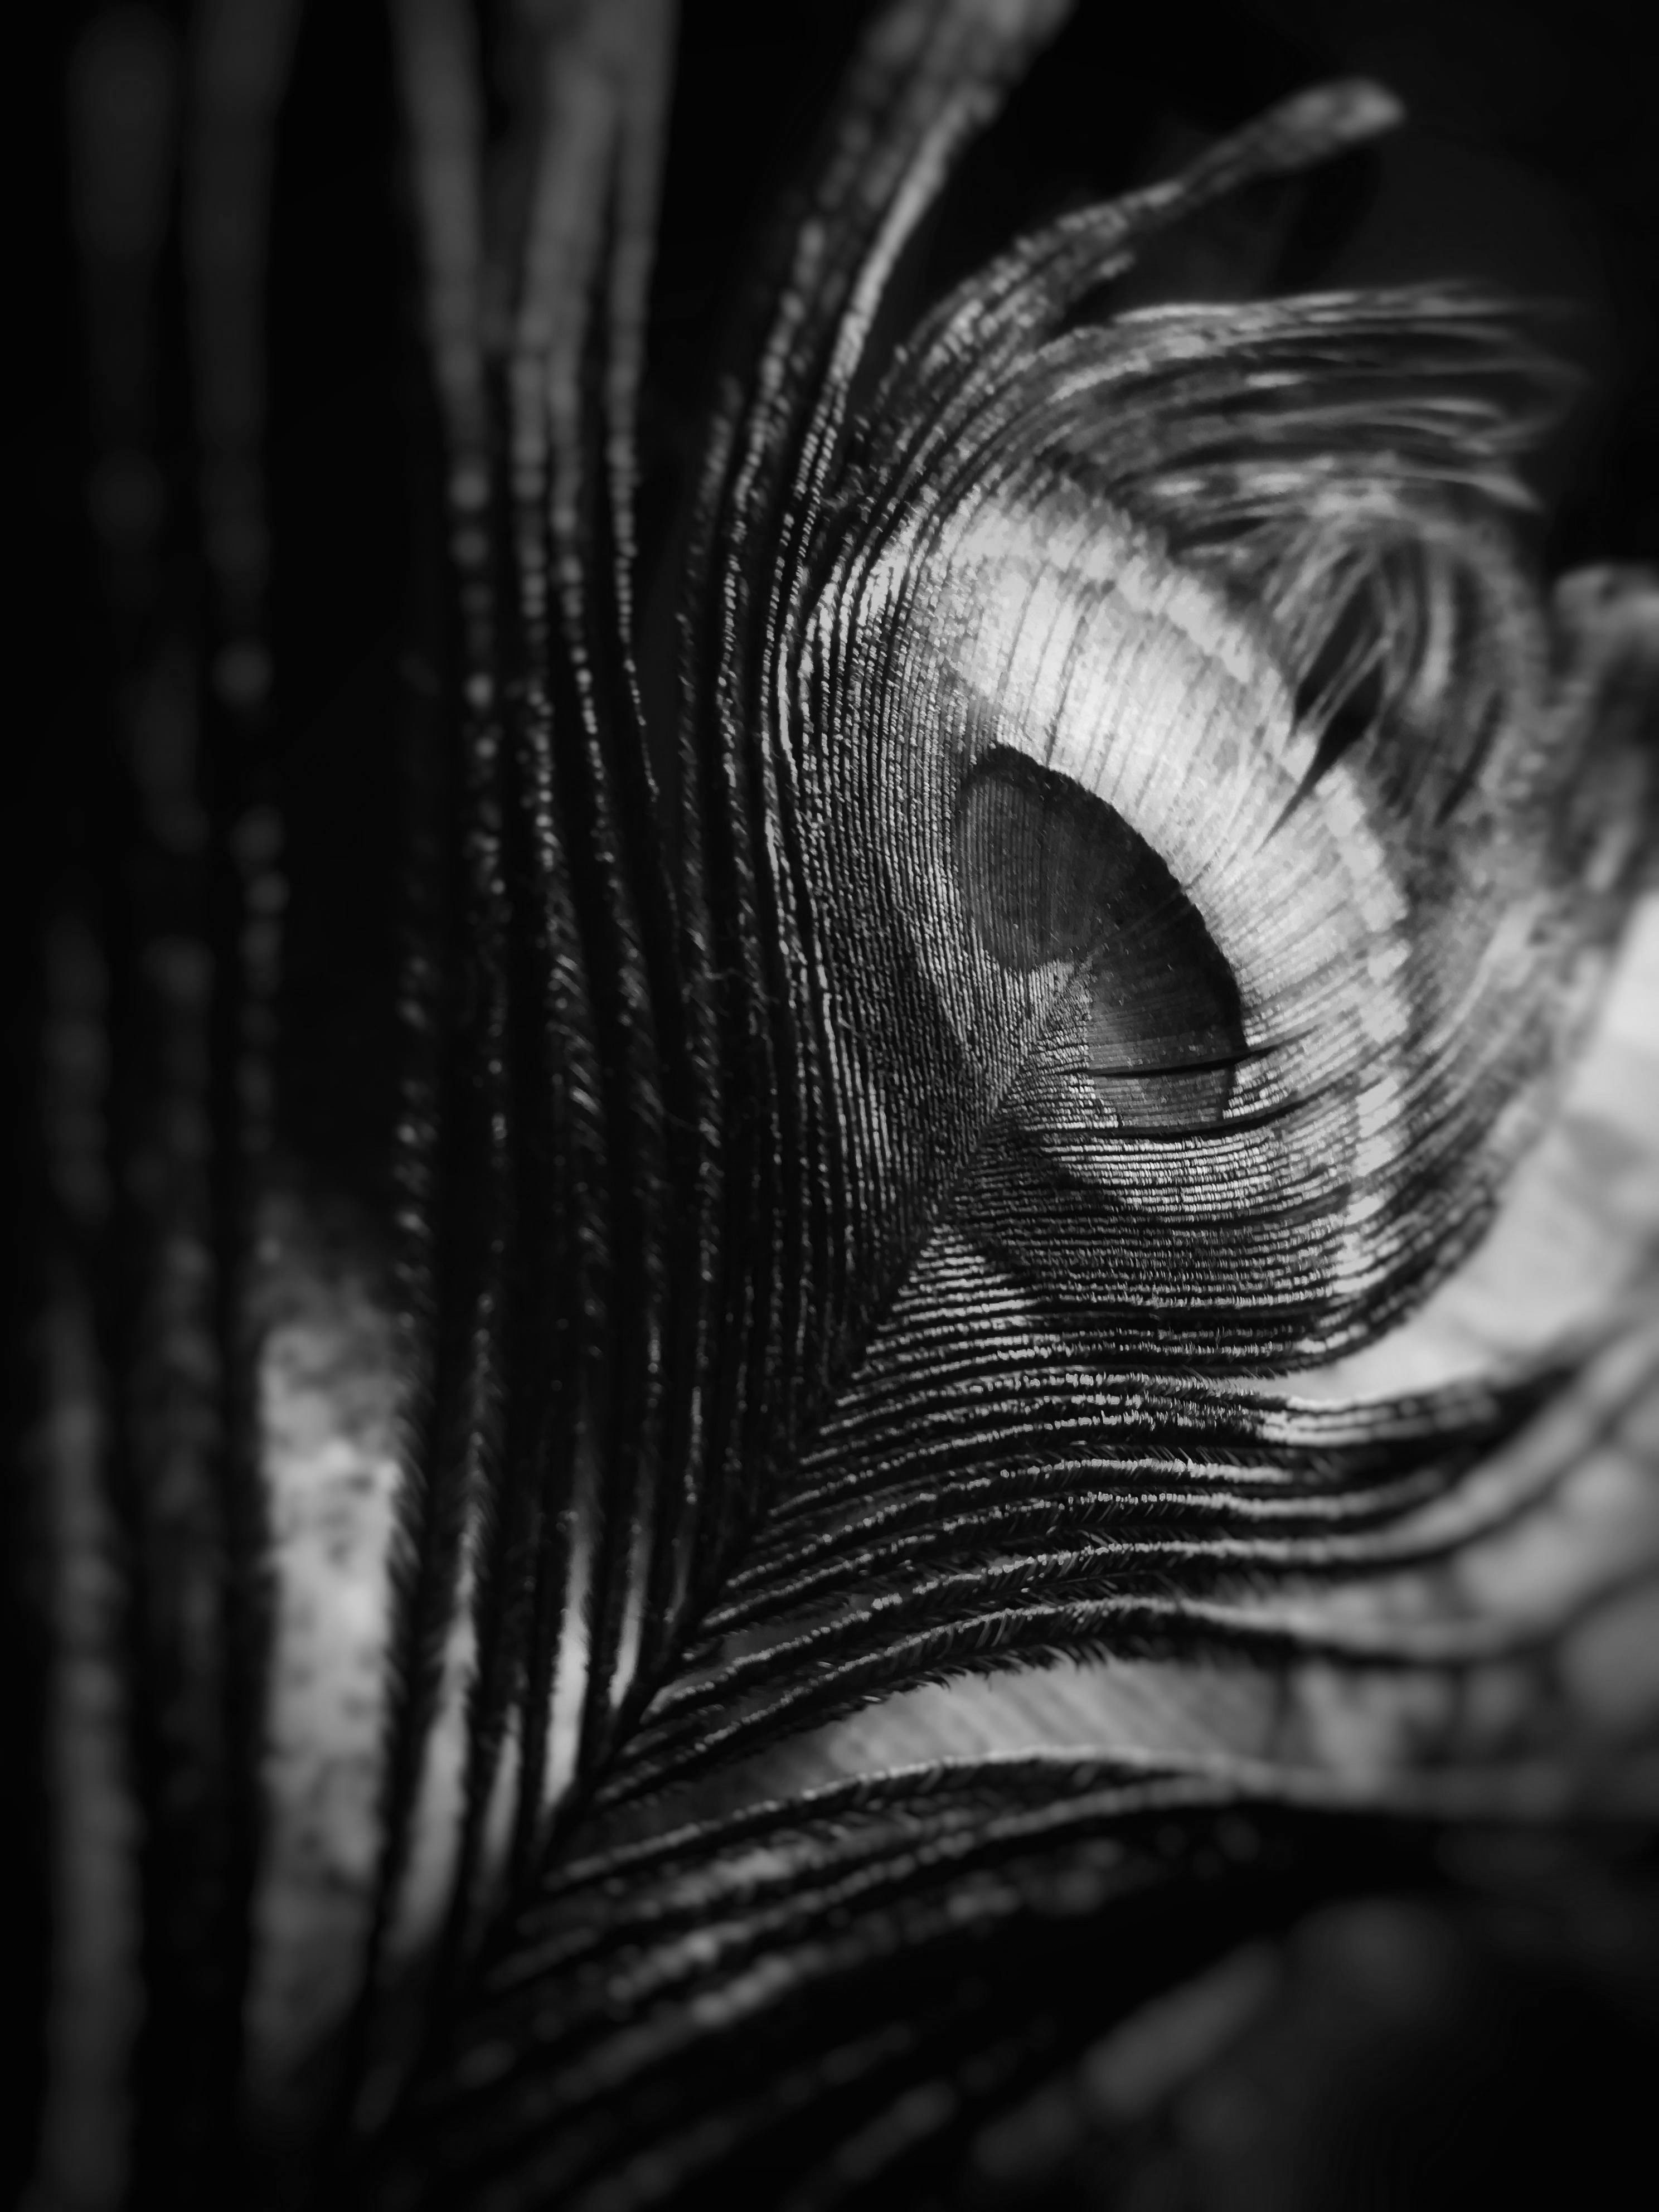
\includegraphics[width=\textwidth]{output/feather_grayscale.jpg}
        \caption{Grayscale}
    \end{subfigure}
    \hfill
    \begin{subfigure}[b]{.225\textwidth}
        \centering
        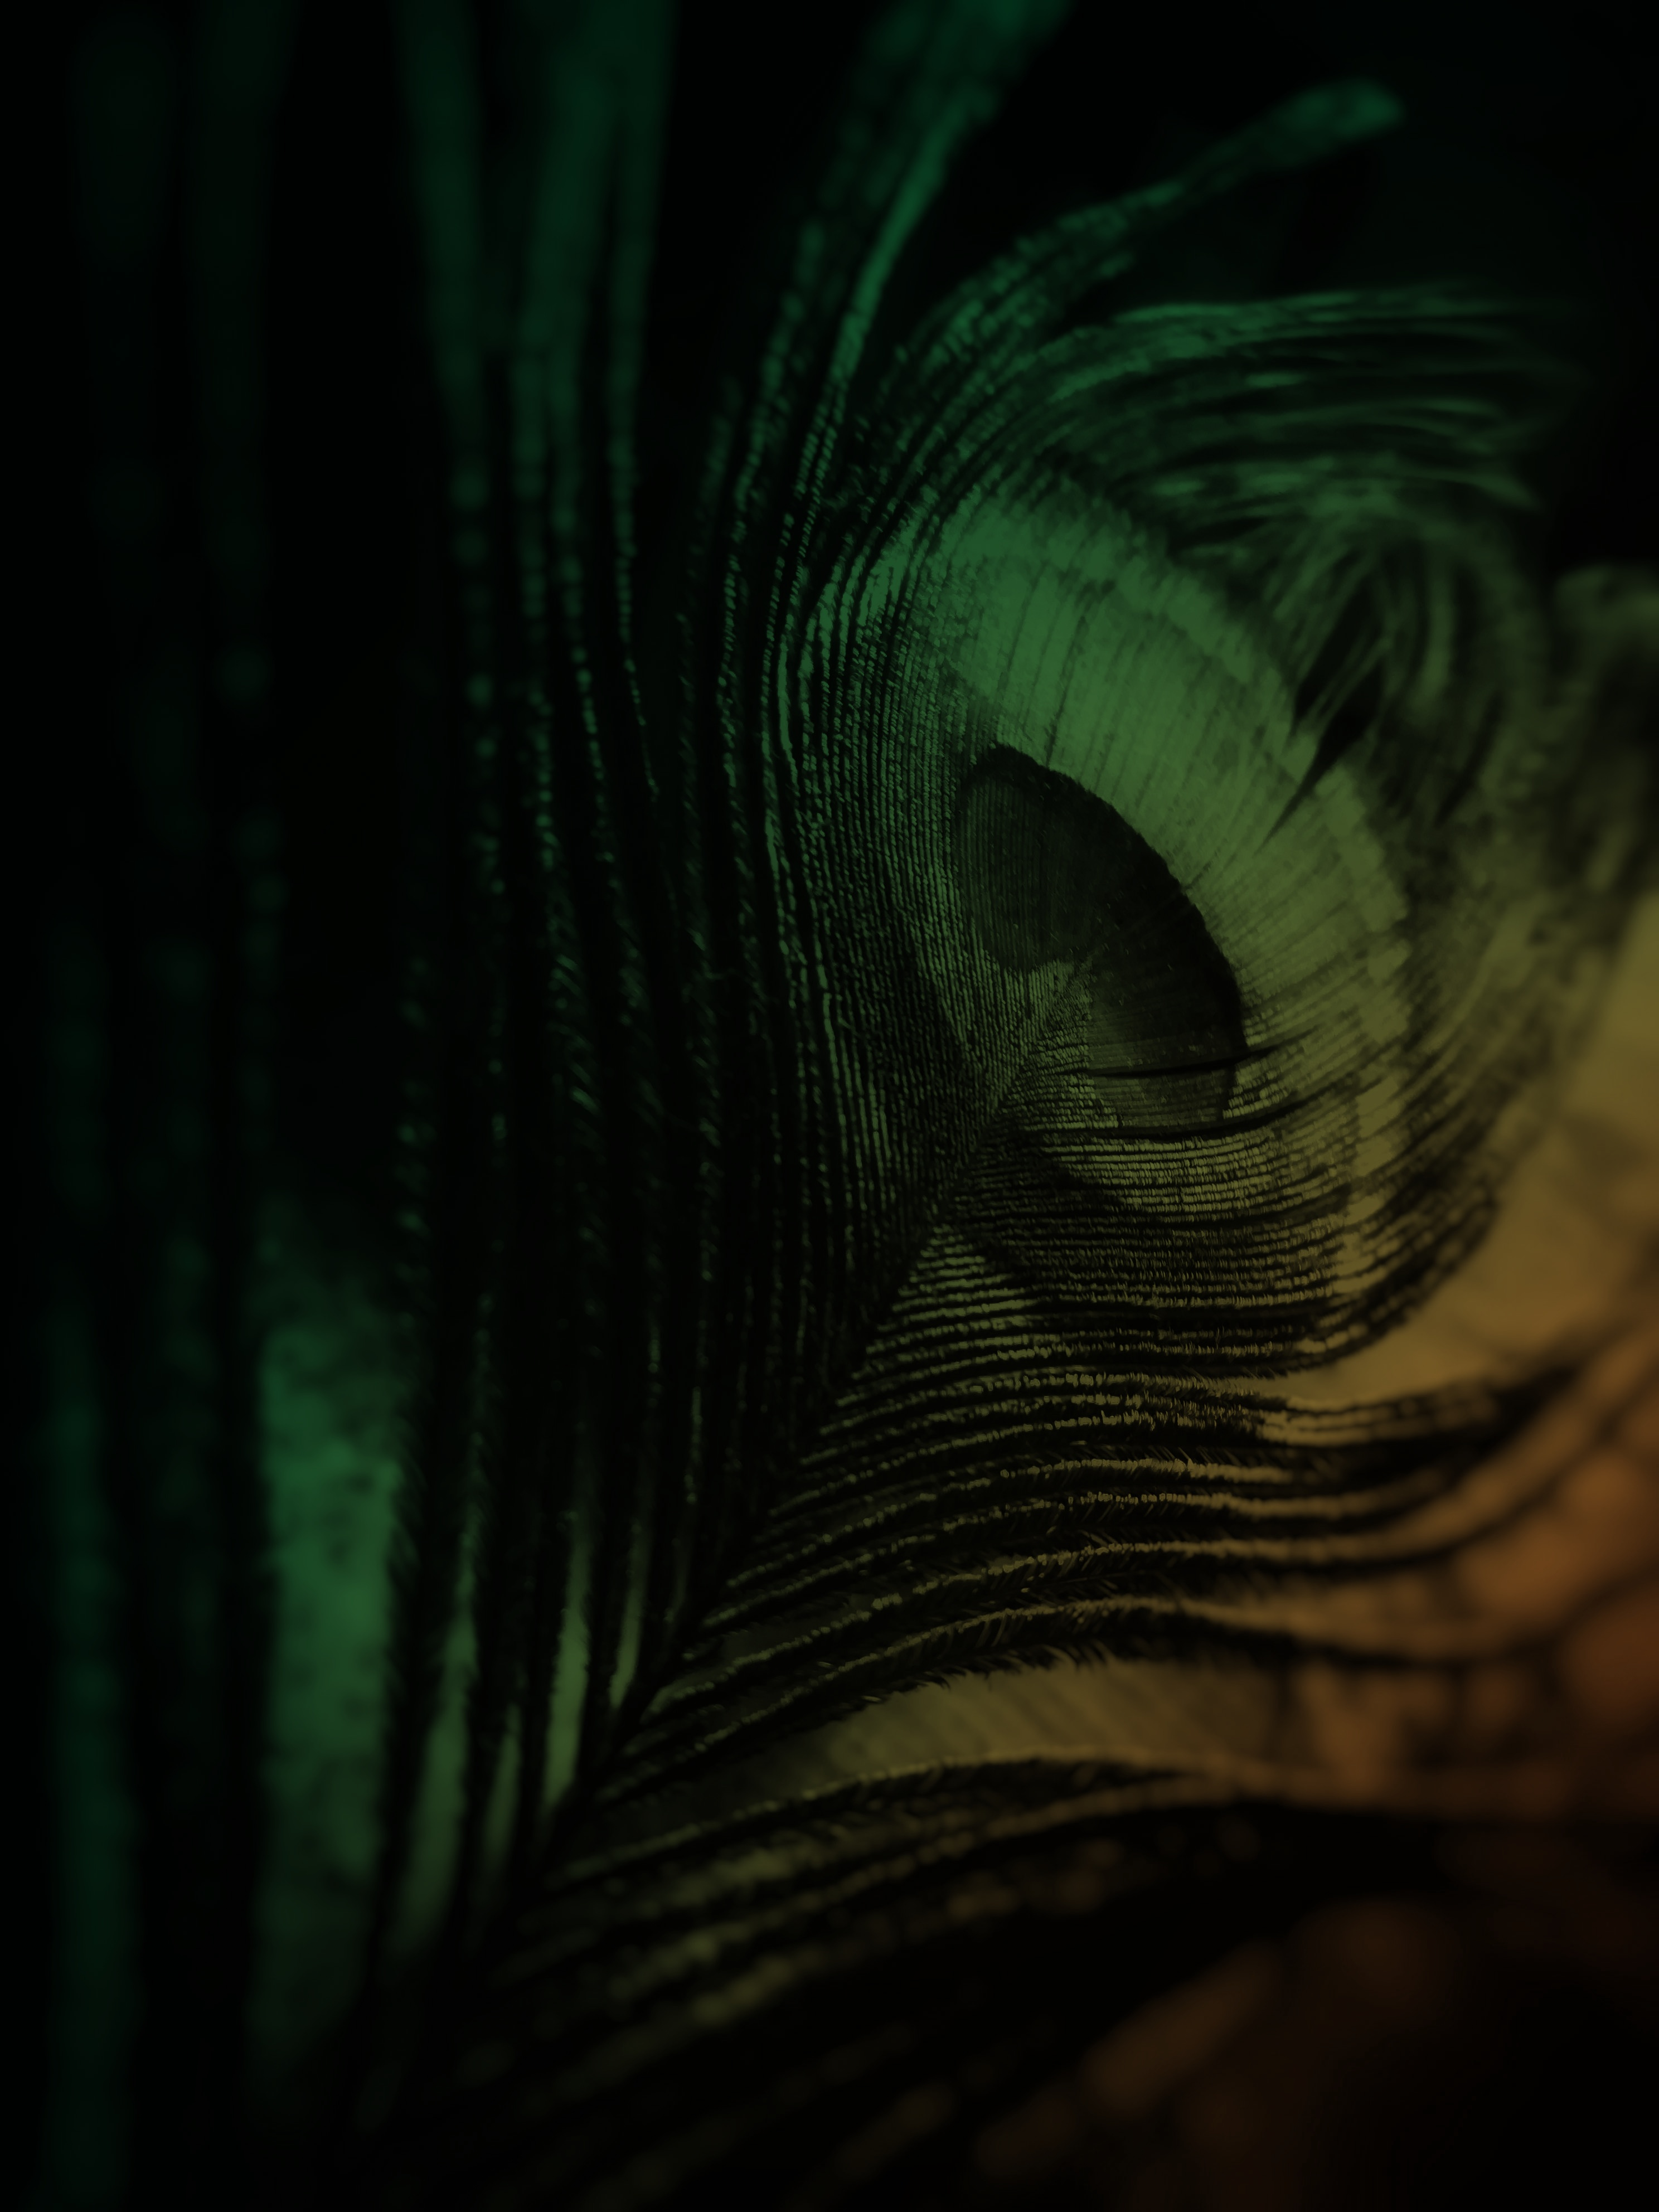
\includegraphics[width=\textwidth]{output/feather_pseudo_colored.jpg}
        \caption{Pseudo Coloring}
    \end{subfigure}
    \hfill
    \begin{subfigure}[b]{.225\textwidth}
        \centering
        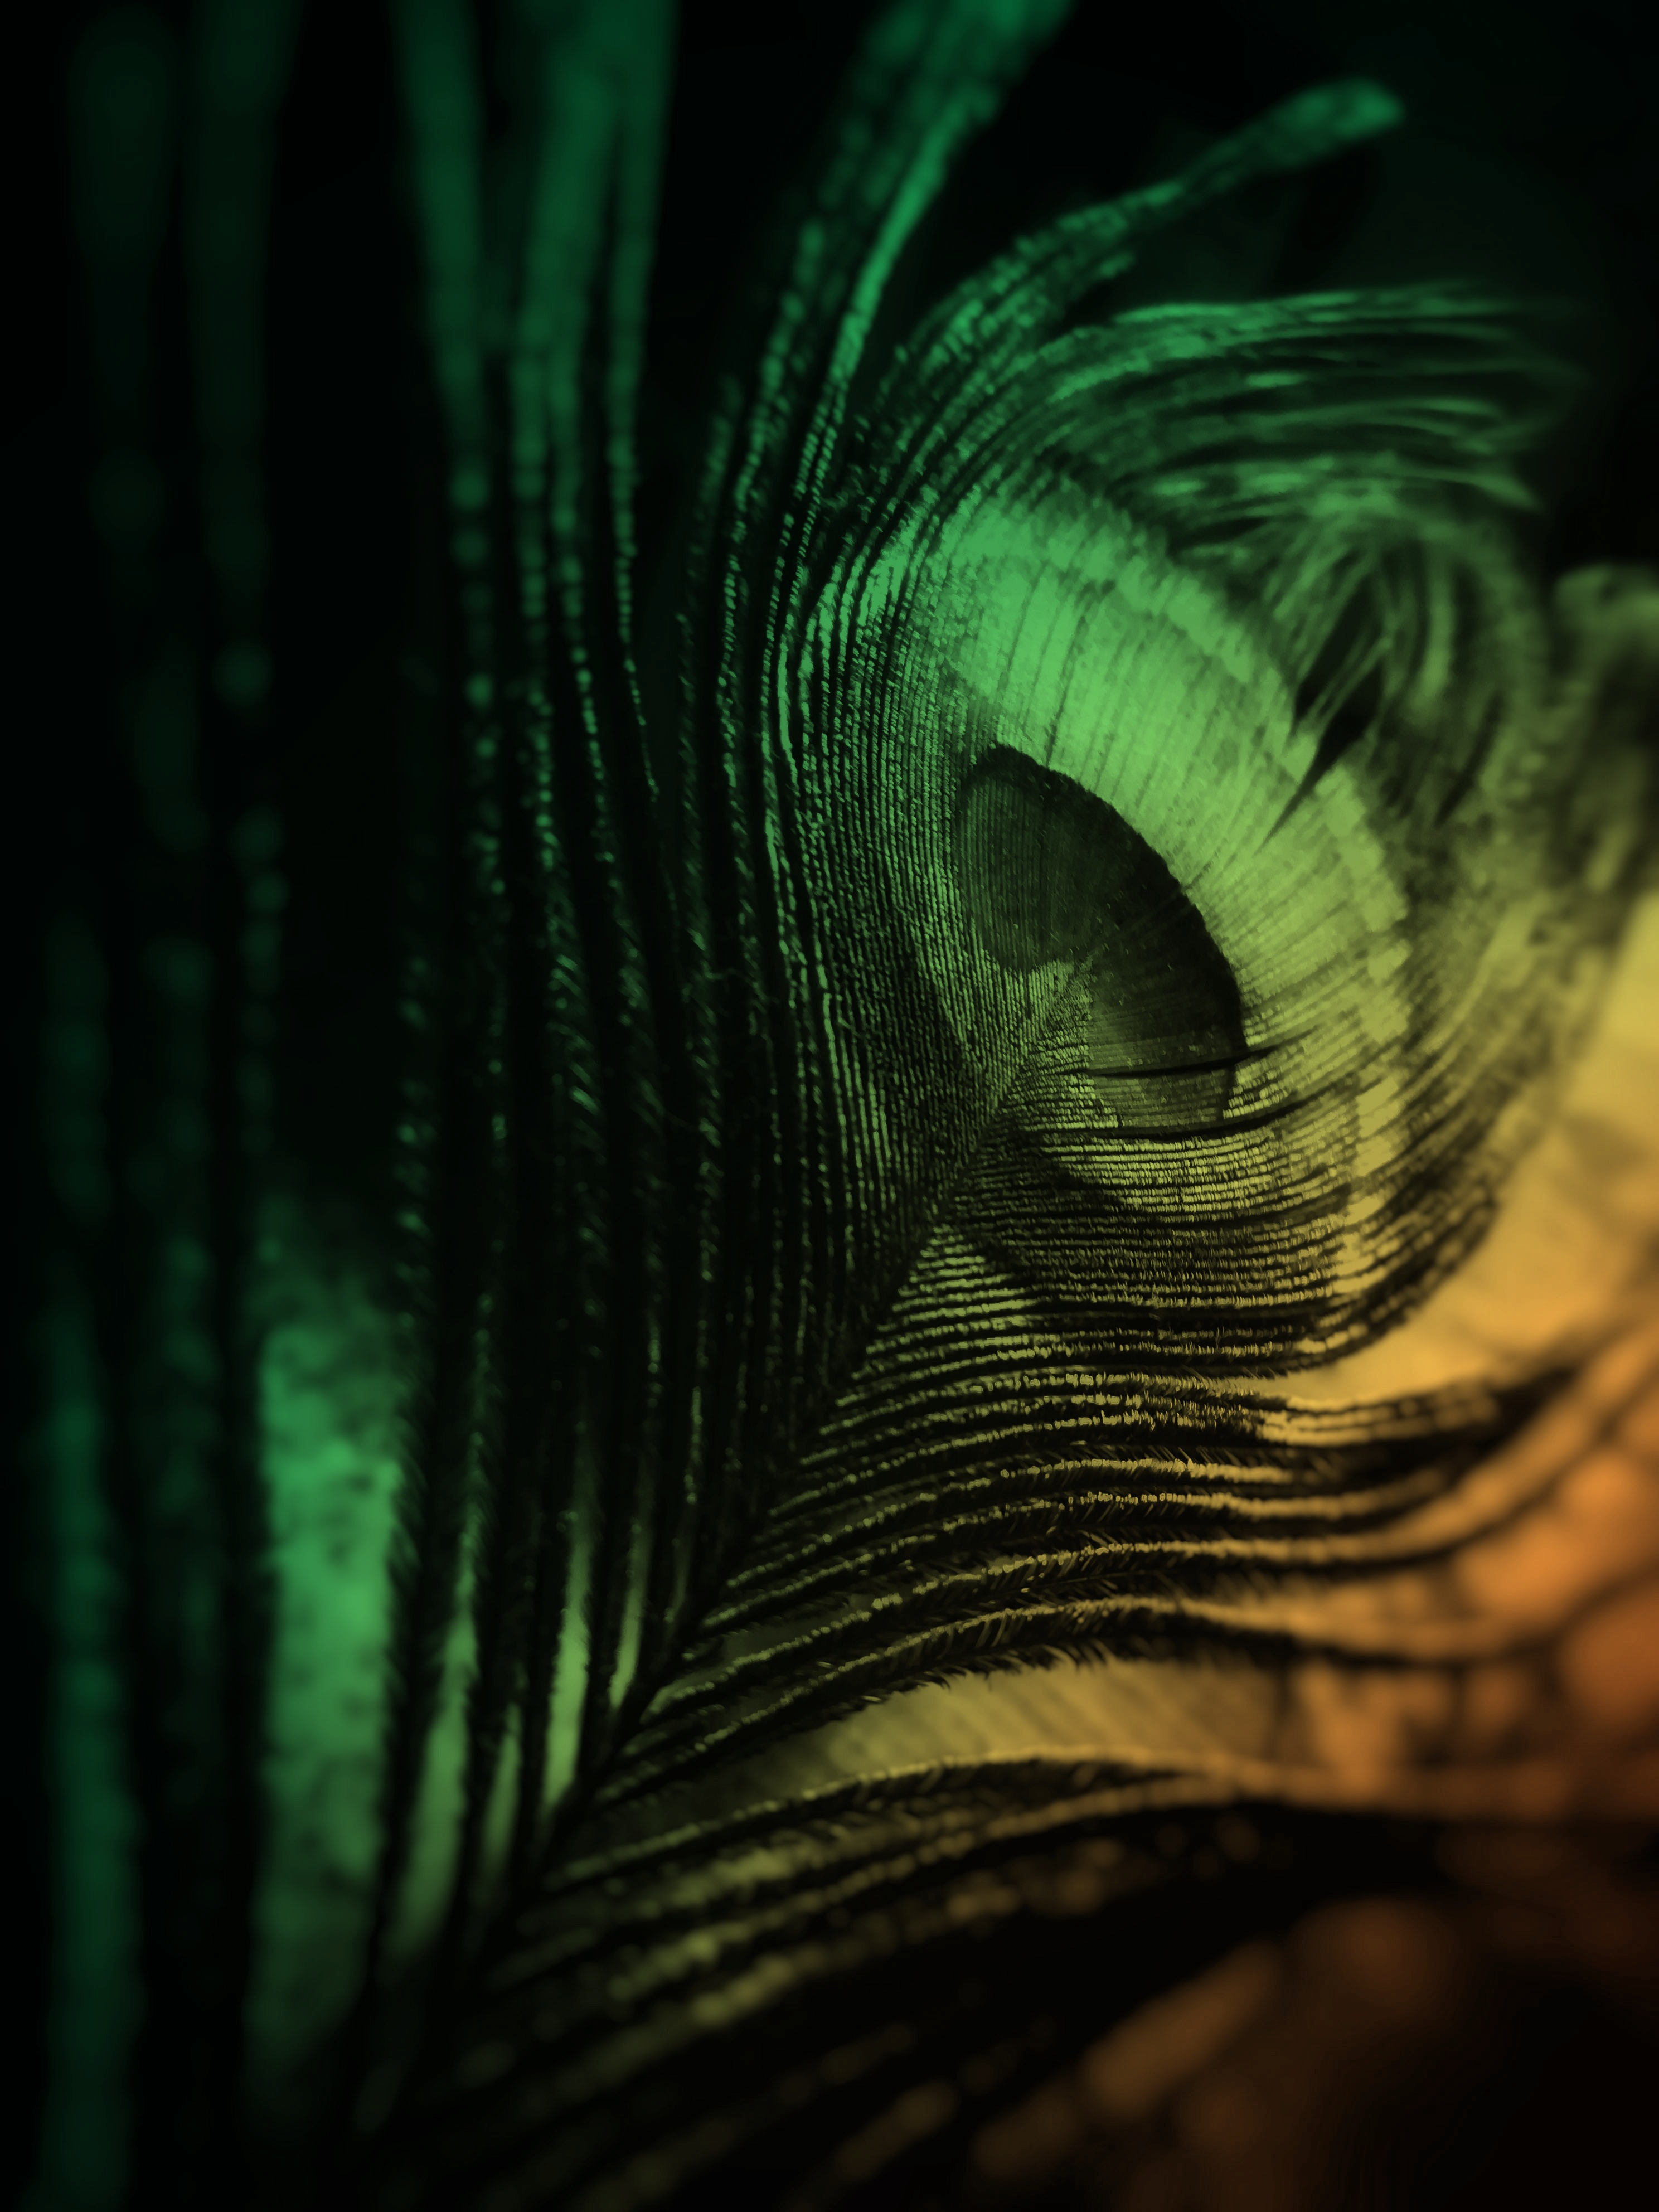
\includegraphics[width=\textwidth]{output/feather_brightness_adjusted.jpg}
        \caption{Brightness * 2}
    \end{subfigure}
    \hfill
    \caption{Pseudo color mapping, after grayscale conversion (70\% green) described earlier.}
    \label{fig:pseudo_color}
\end{figure}

\section{Chroma Keying}

For chroma keying, we first resize the foreground image to blend perfectly in the background. We specifically superpose those pixels on the background where the ratio of green channel's intensity exceeds a threshold times that of red or blue channel.

\begin{figure}[H]
    \hfill
    \centering
    \begin{subfigure}[b]{.3\textwidth}
        \centering
        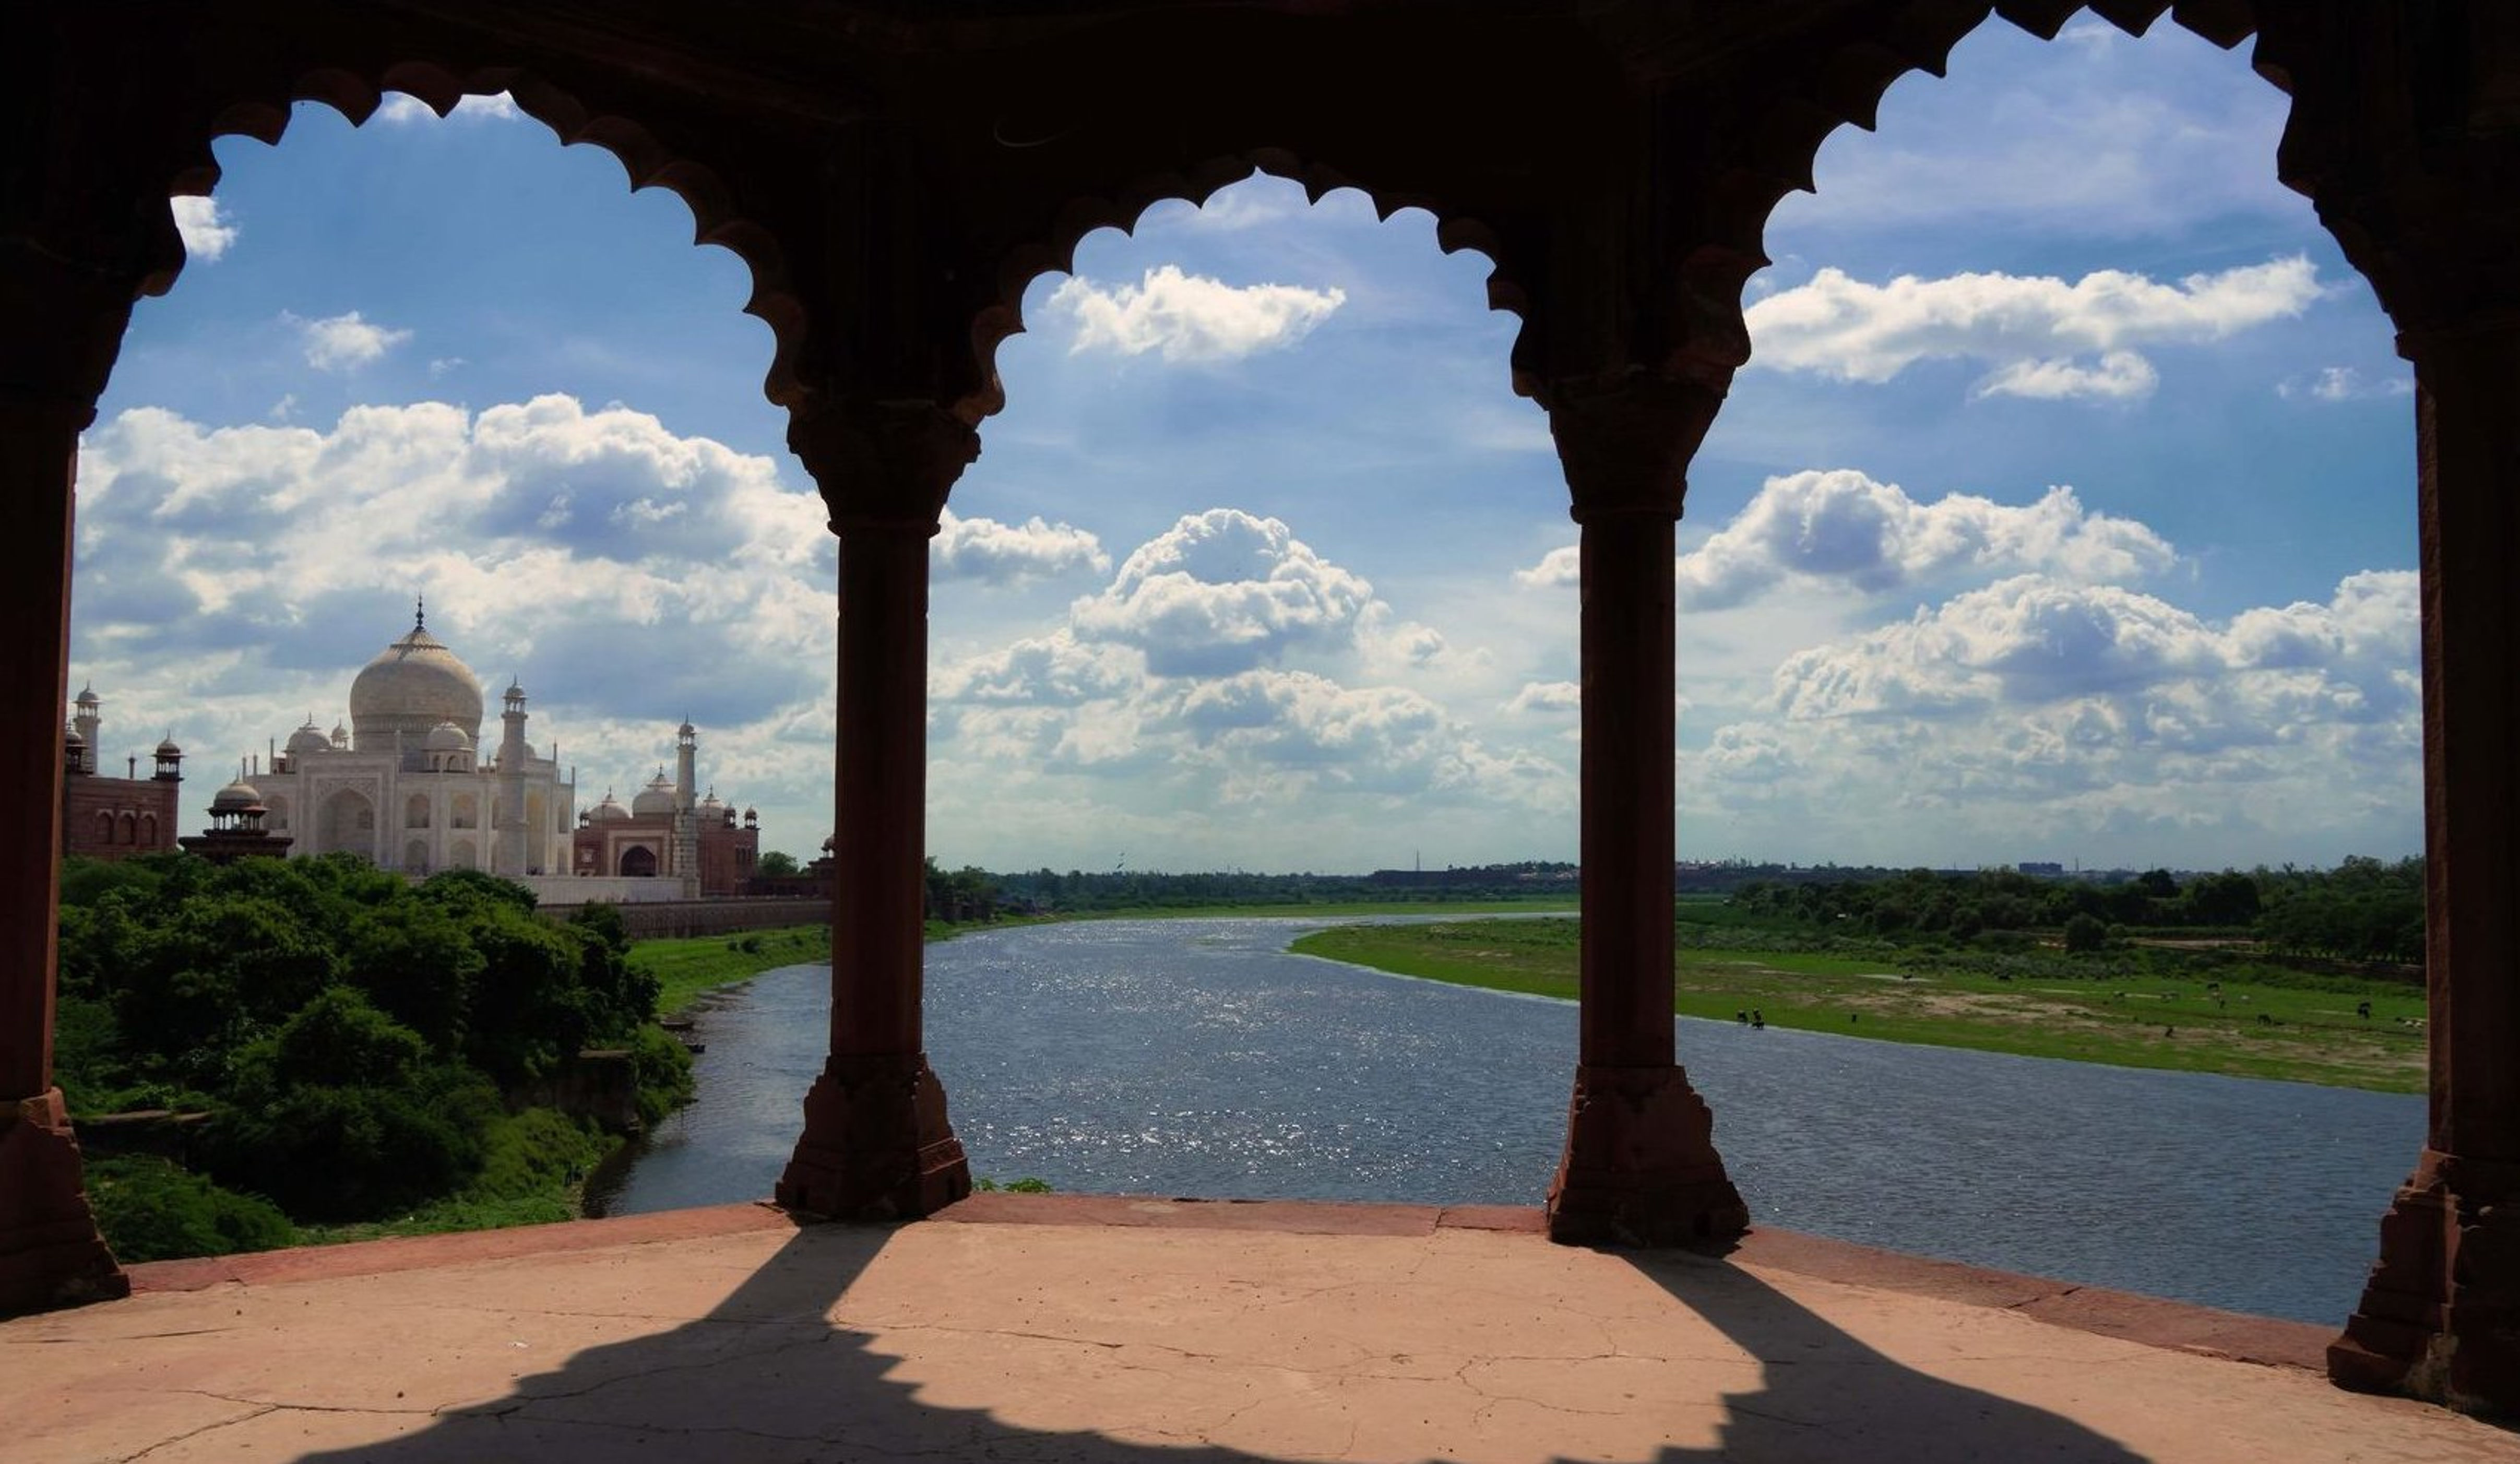
\includegraphics[width=\textwidth]{media/tajmahal.jpg}
        \caption{Background}
    \end{subfigure}
    \hfill
    \begin{subfigure}[b]{.3\textwidth}
        \centering
        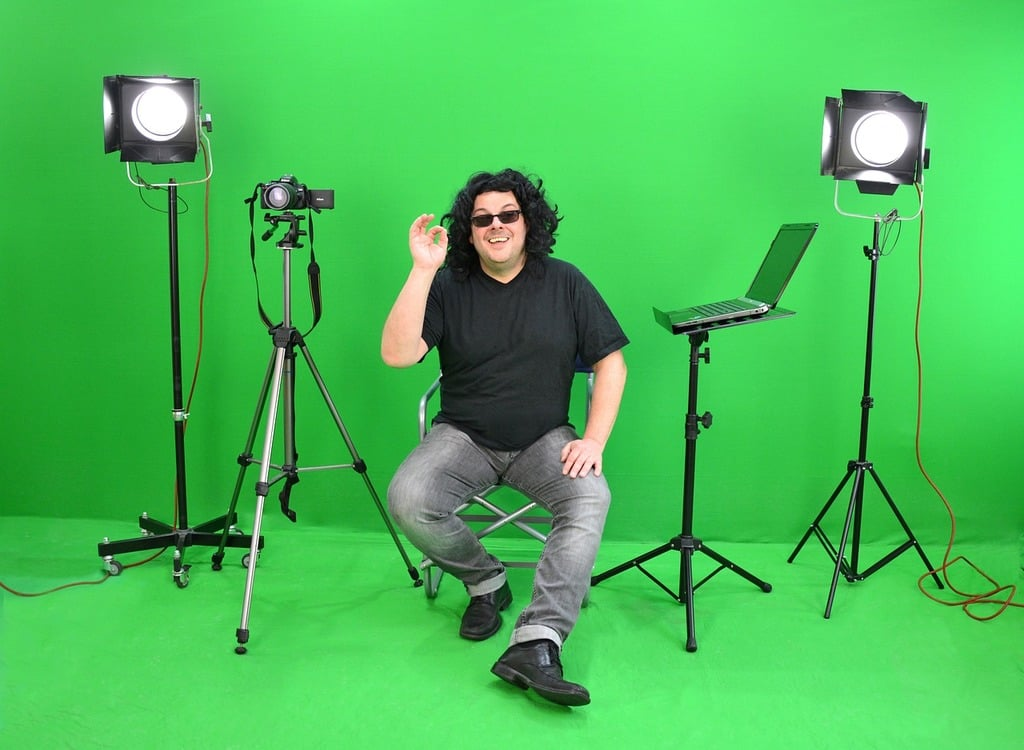
\includegraphics[width=\textwidth]{media/greenbox-director.jpg}
        \caption{Foreground}
    \end{subfigure}
    \hfill
    \begin{subfigure}[b]{.3\textwidth}
        \centering
        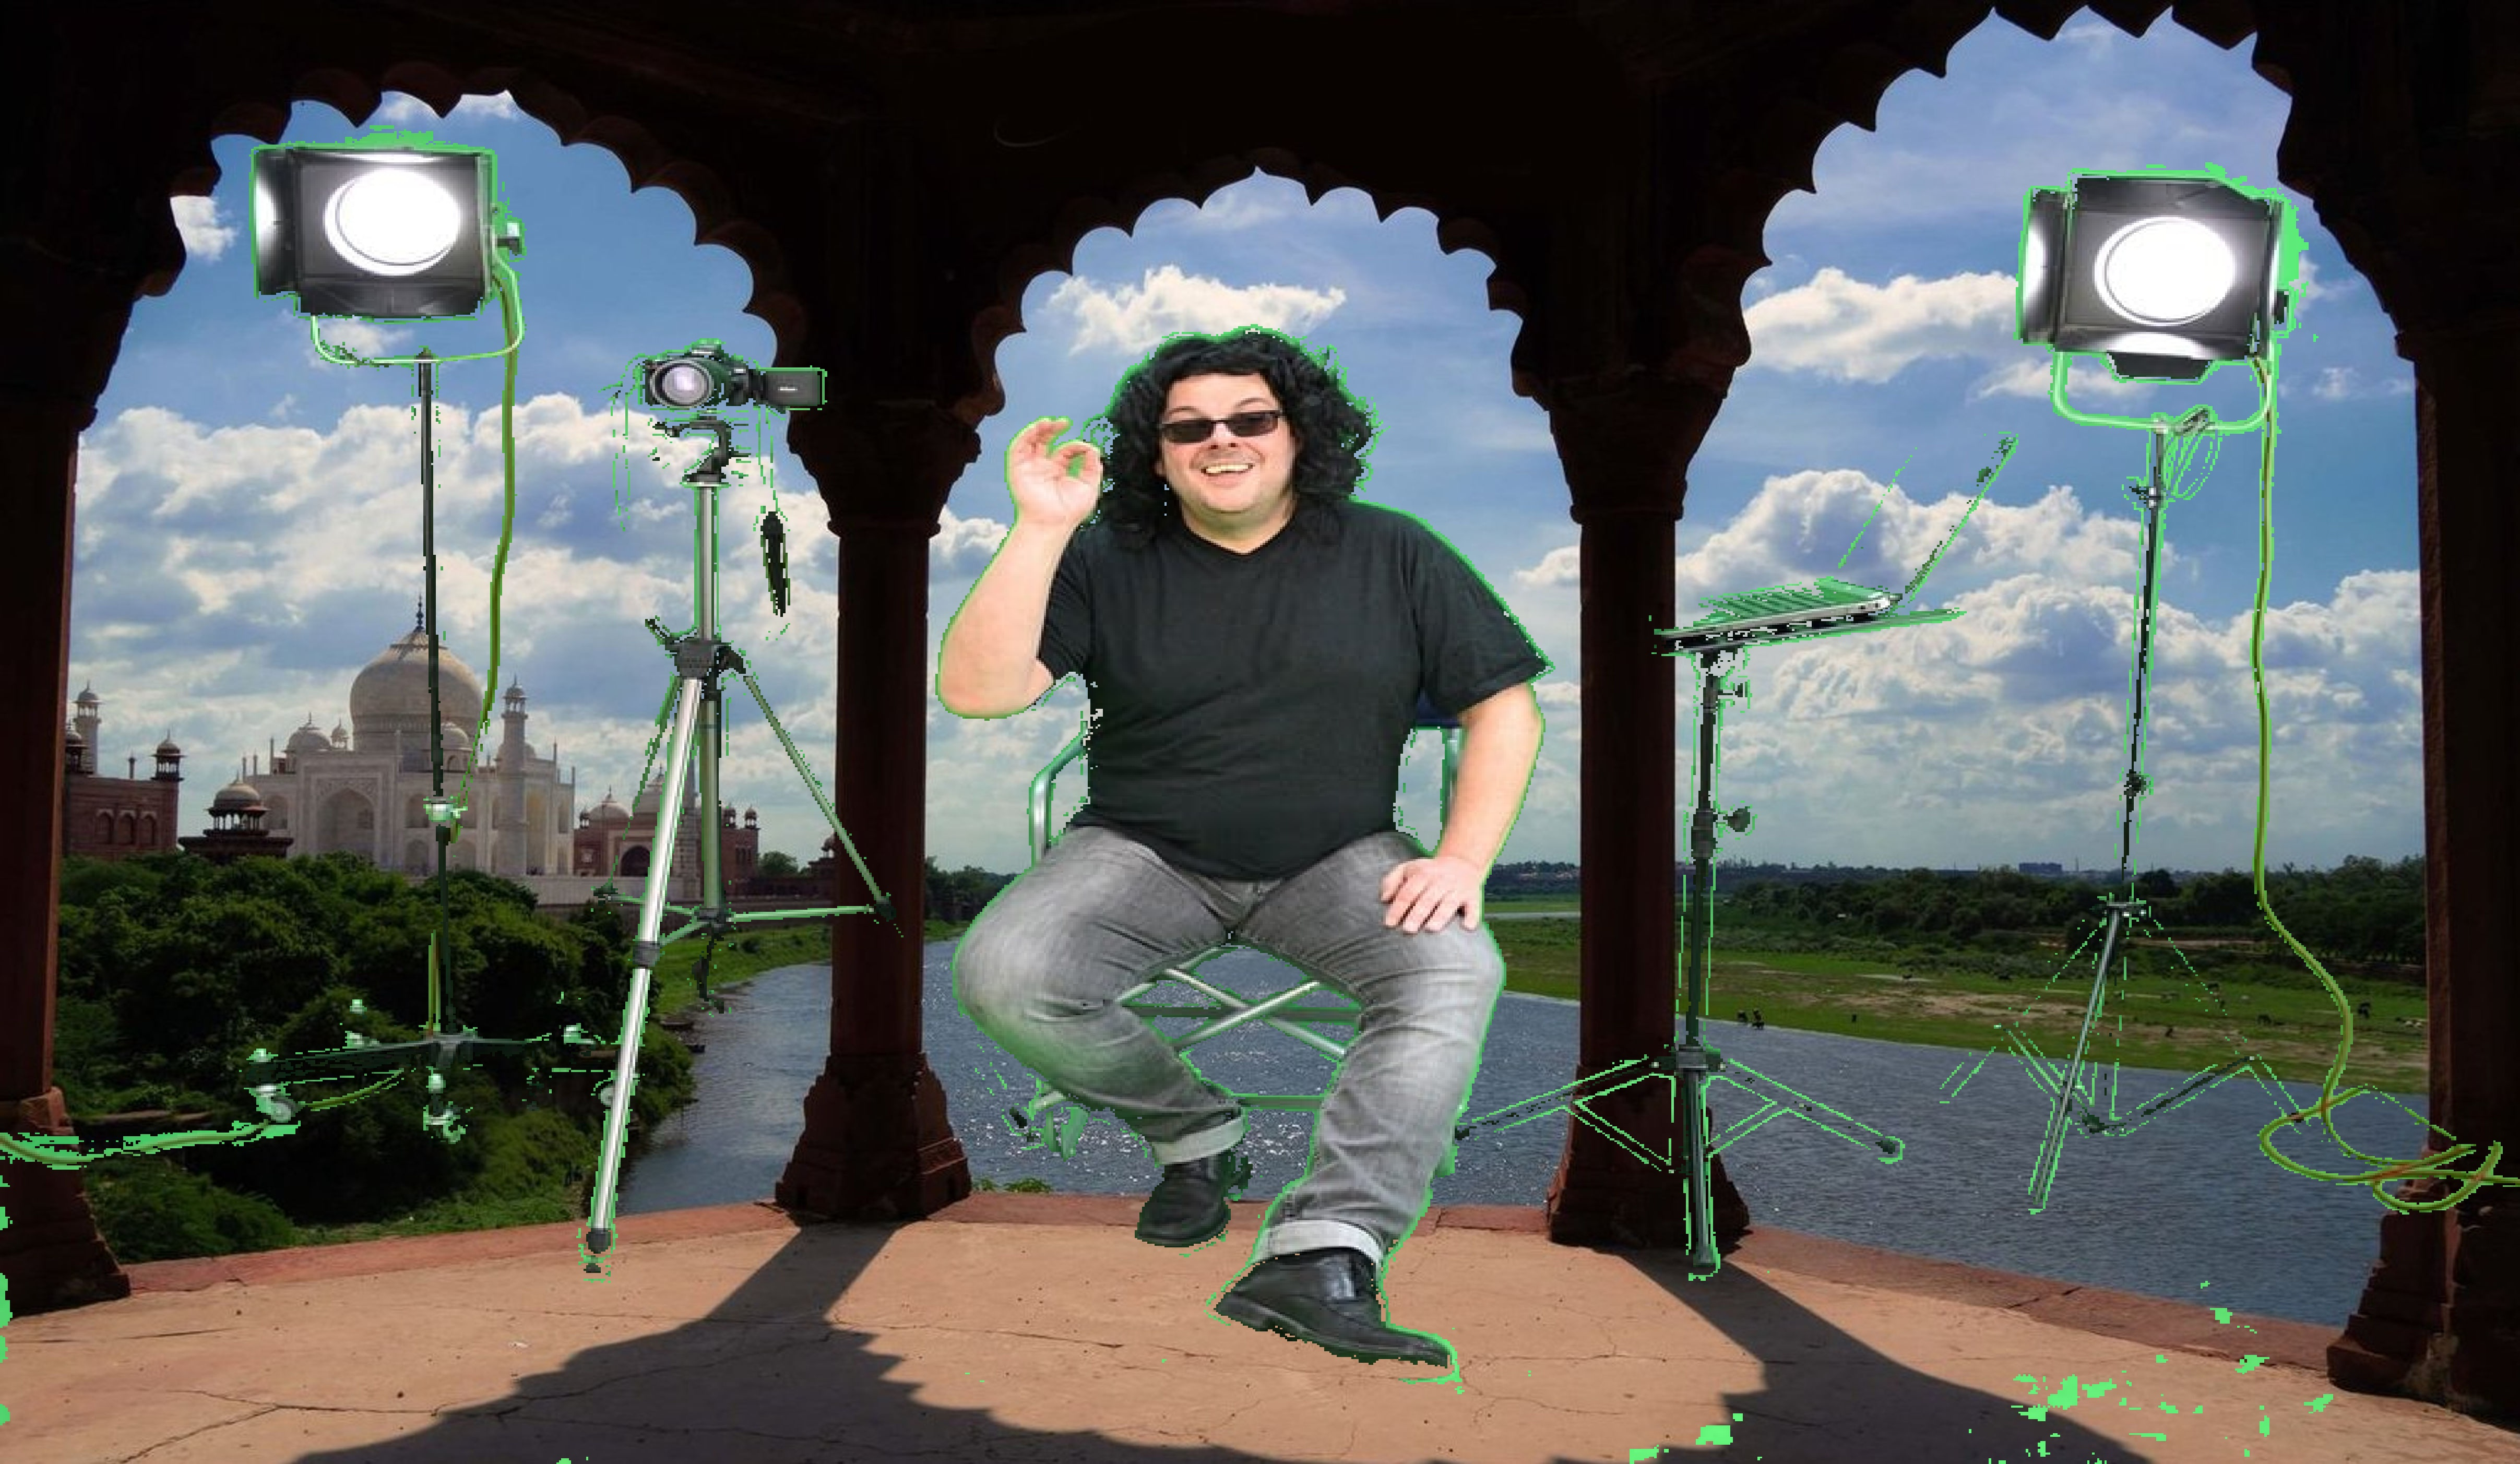
\includegraphics[width=\textwidth]{output/chroma_keying.jpg}
        \caption{Merge}
    \end{subfigure}
    \hfill
    \caption{Chroma keying in RGB color space.}
    \label{fig:chroma_keying}
\end{figure}

\section{Fade Transition}

To demonstrate this, we use the earlier images from Chroma Keying. A simple convex combination with gradual shift in the coefficient, based on time/frame number suffices to emulate a fade transition.

\begin{figure}[H]
    \hfill
    \centering
    \begin{subfigure}[b]{.3\textwidth}
        \centering
        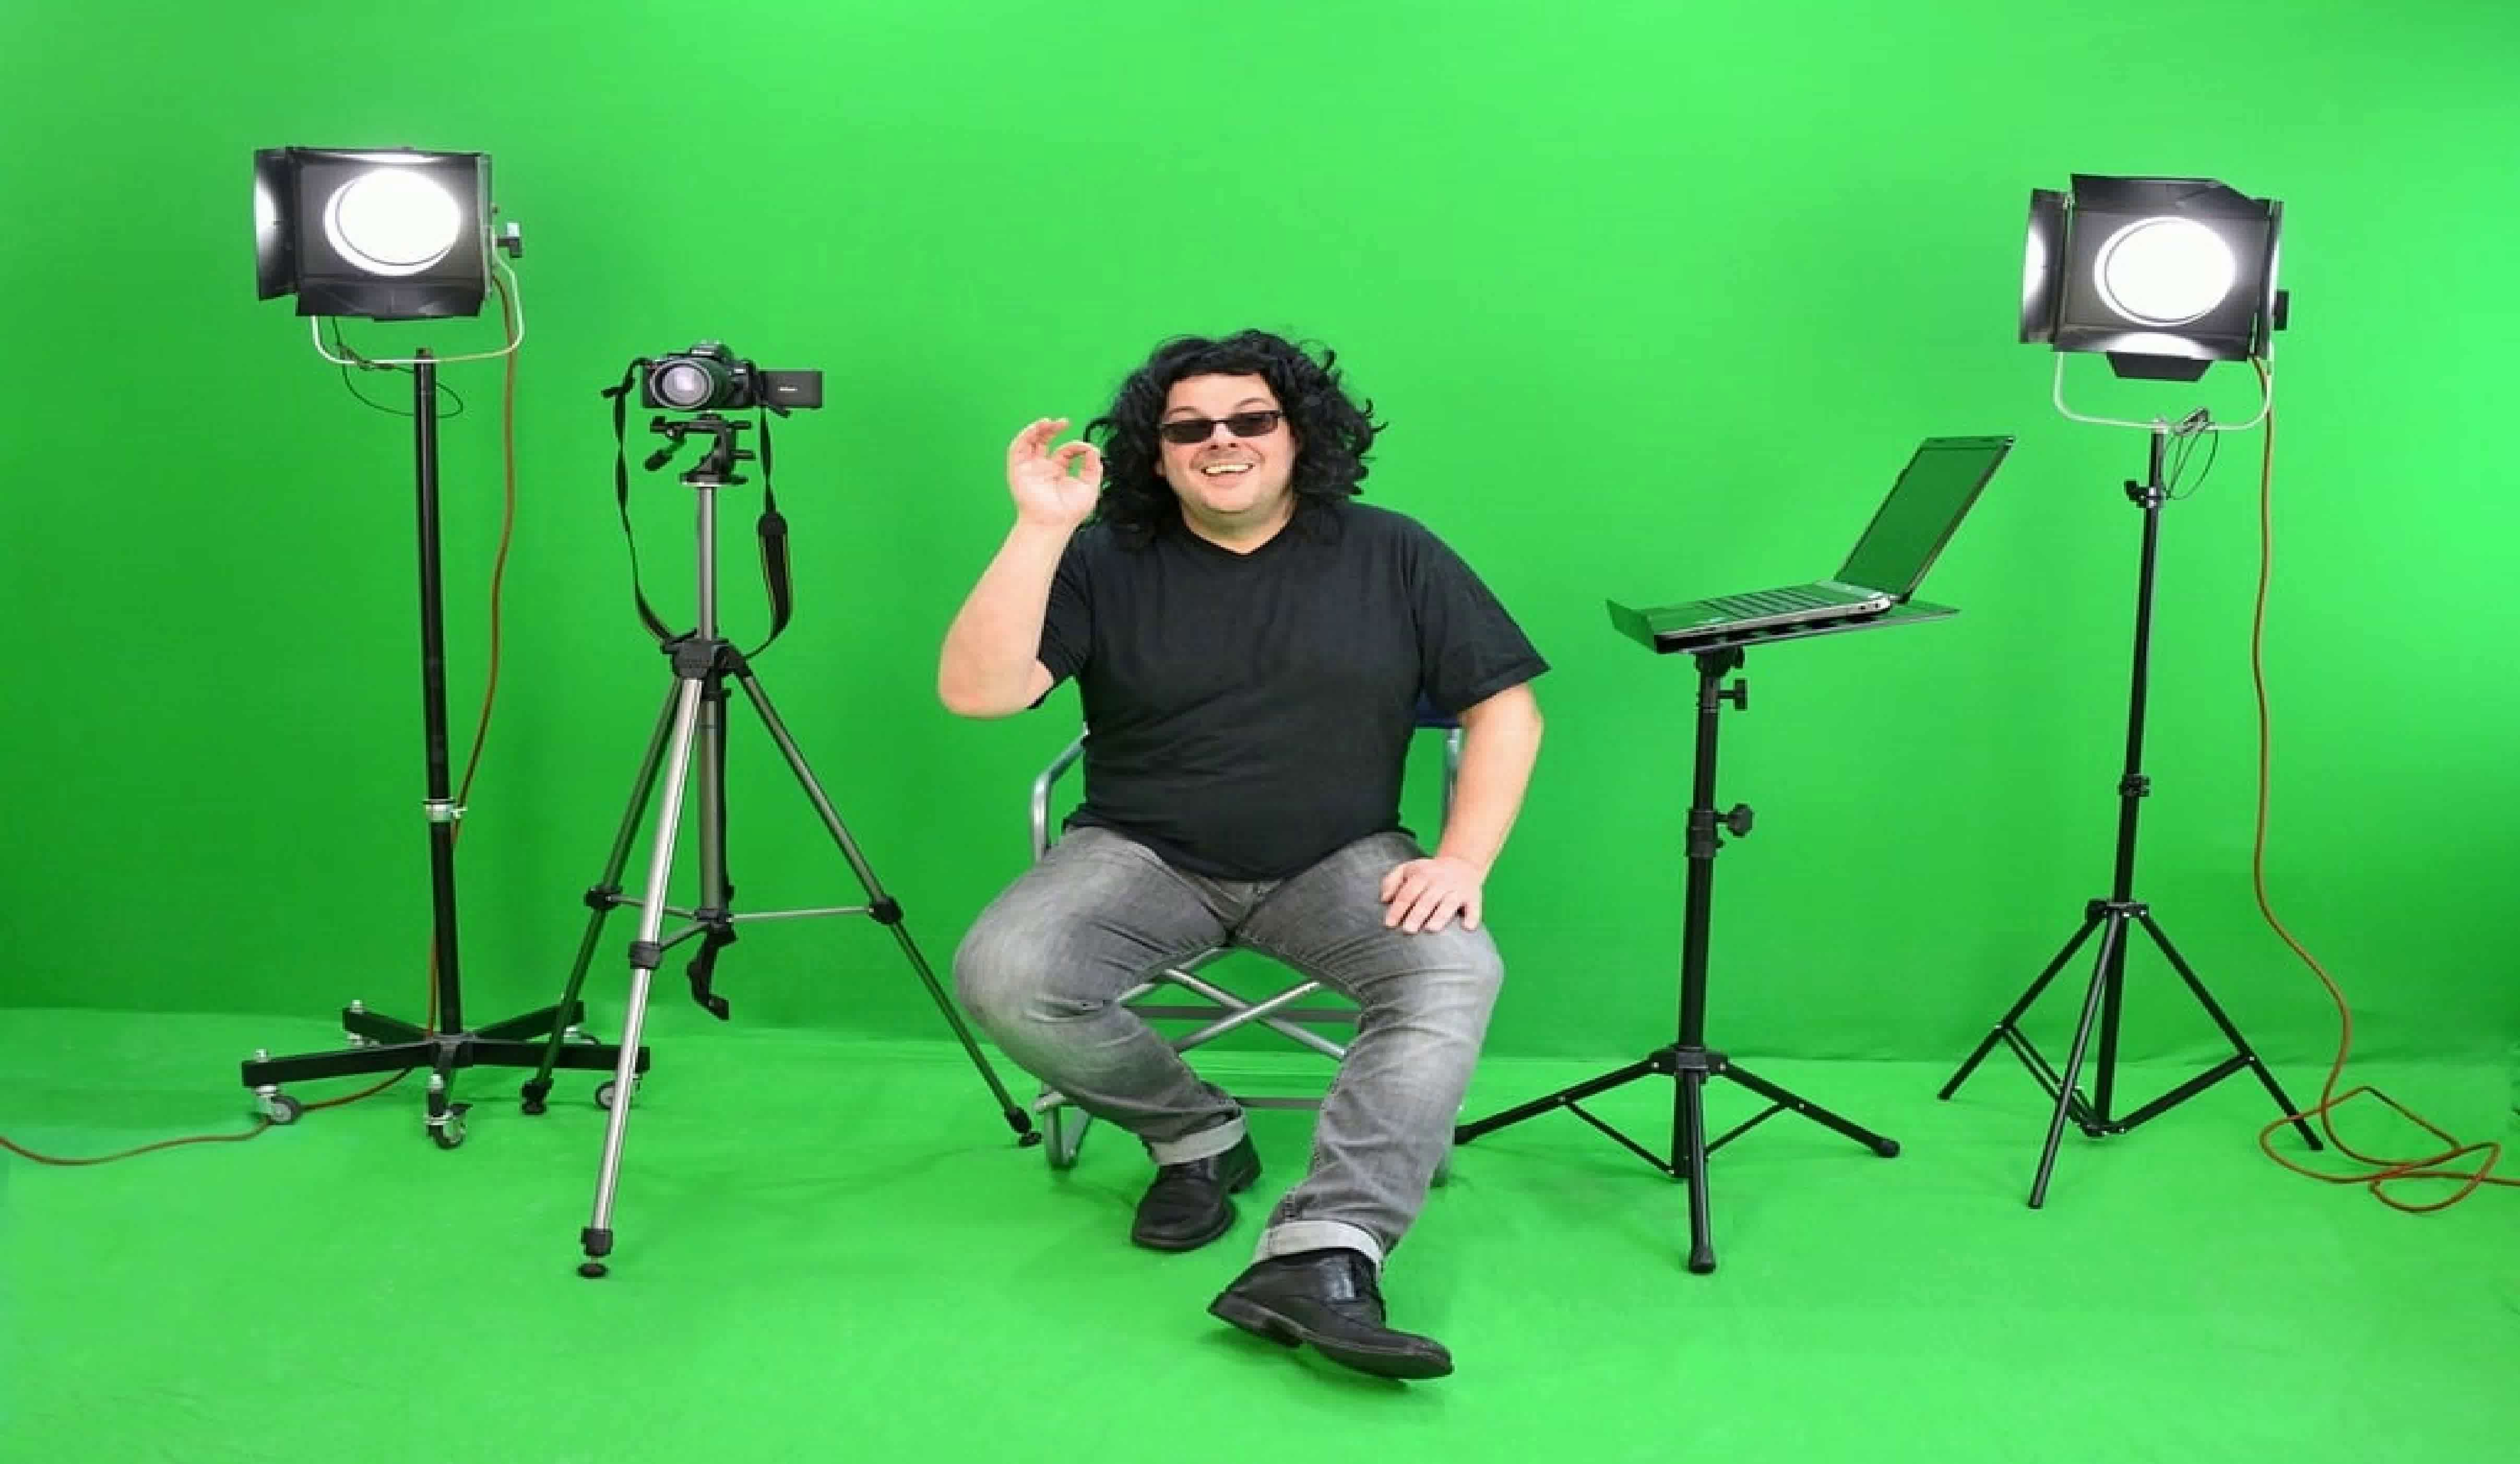
\includegraphics[width=\textwidth]{output/fade_transition_1.jpg}
        \caption{First Frame}
    \end{subfigure}
    \hfill
    \begin{subfigure}[b]{.3\textwidth}
        \centering
        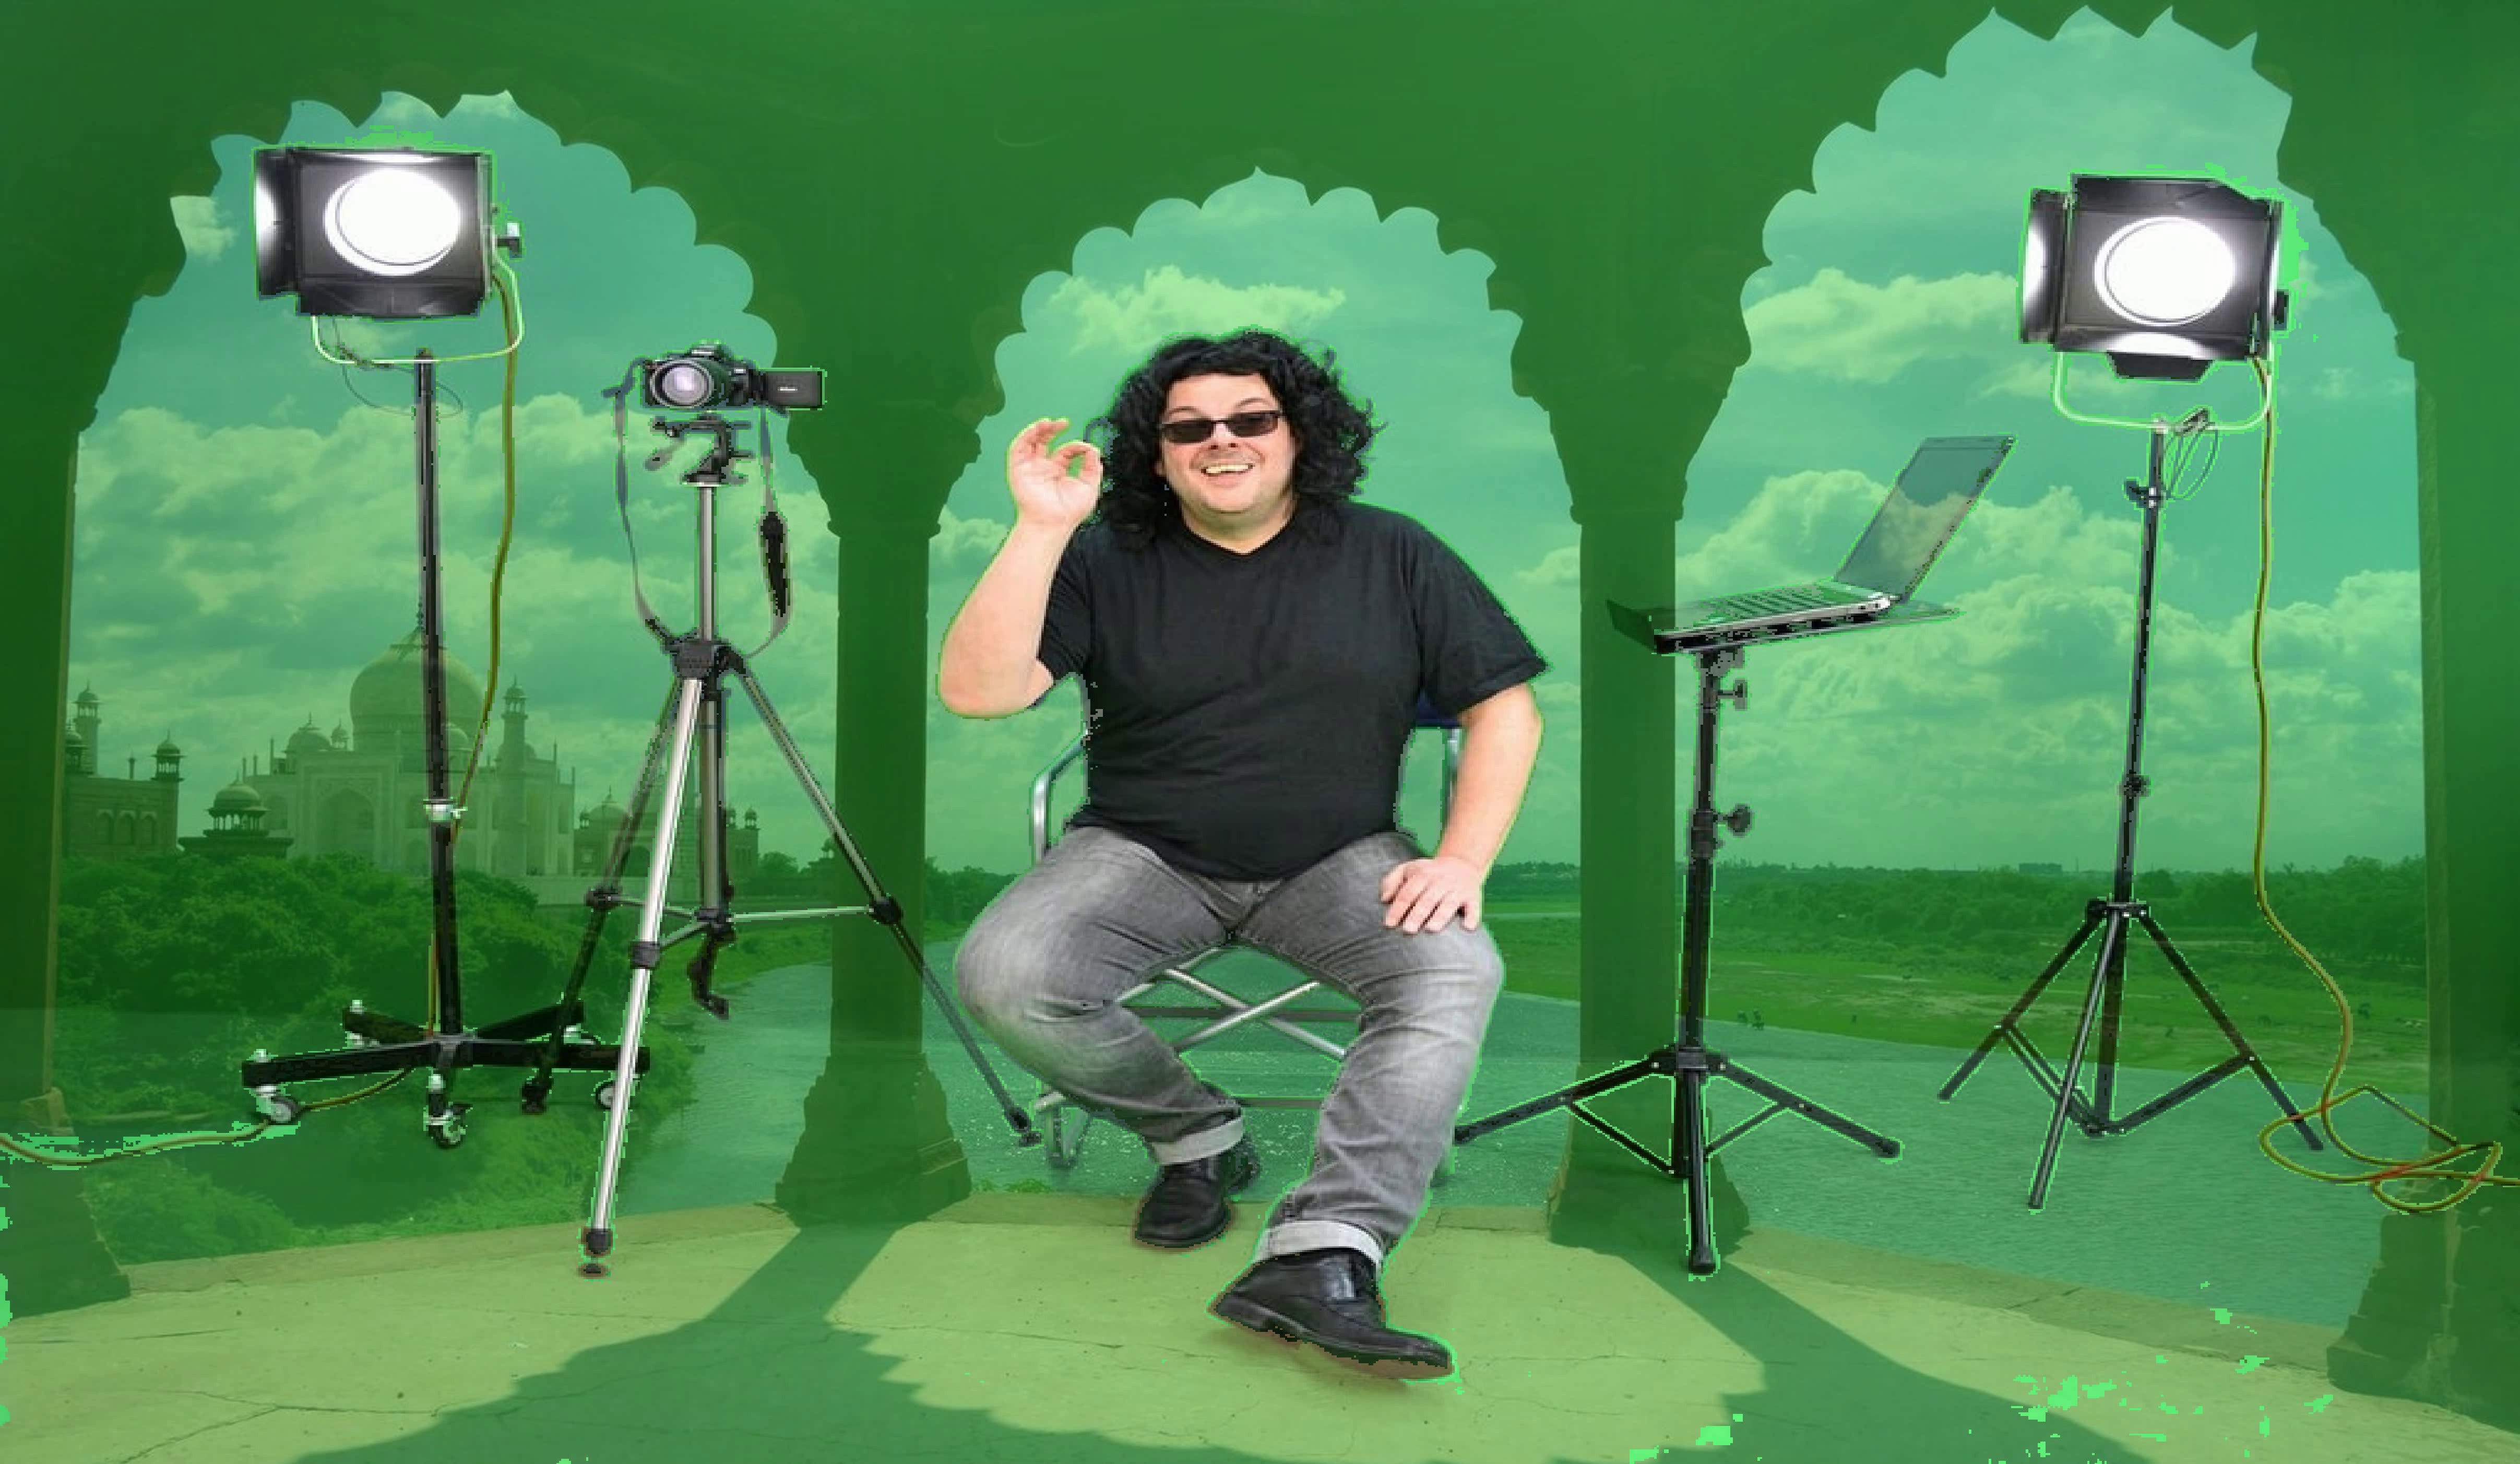
\includegraphics[width=\textwidth]{output/fade_transition_13.jpg}
        \caption{Intermediate Frame}
    \end{subfigure}
    \hfill
    \begin{subfigure}[b]{.3\textwidth}
        \centering
        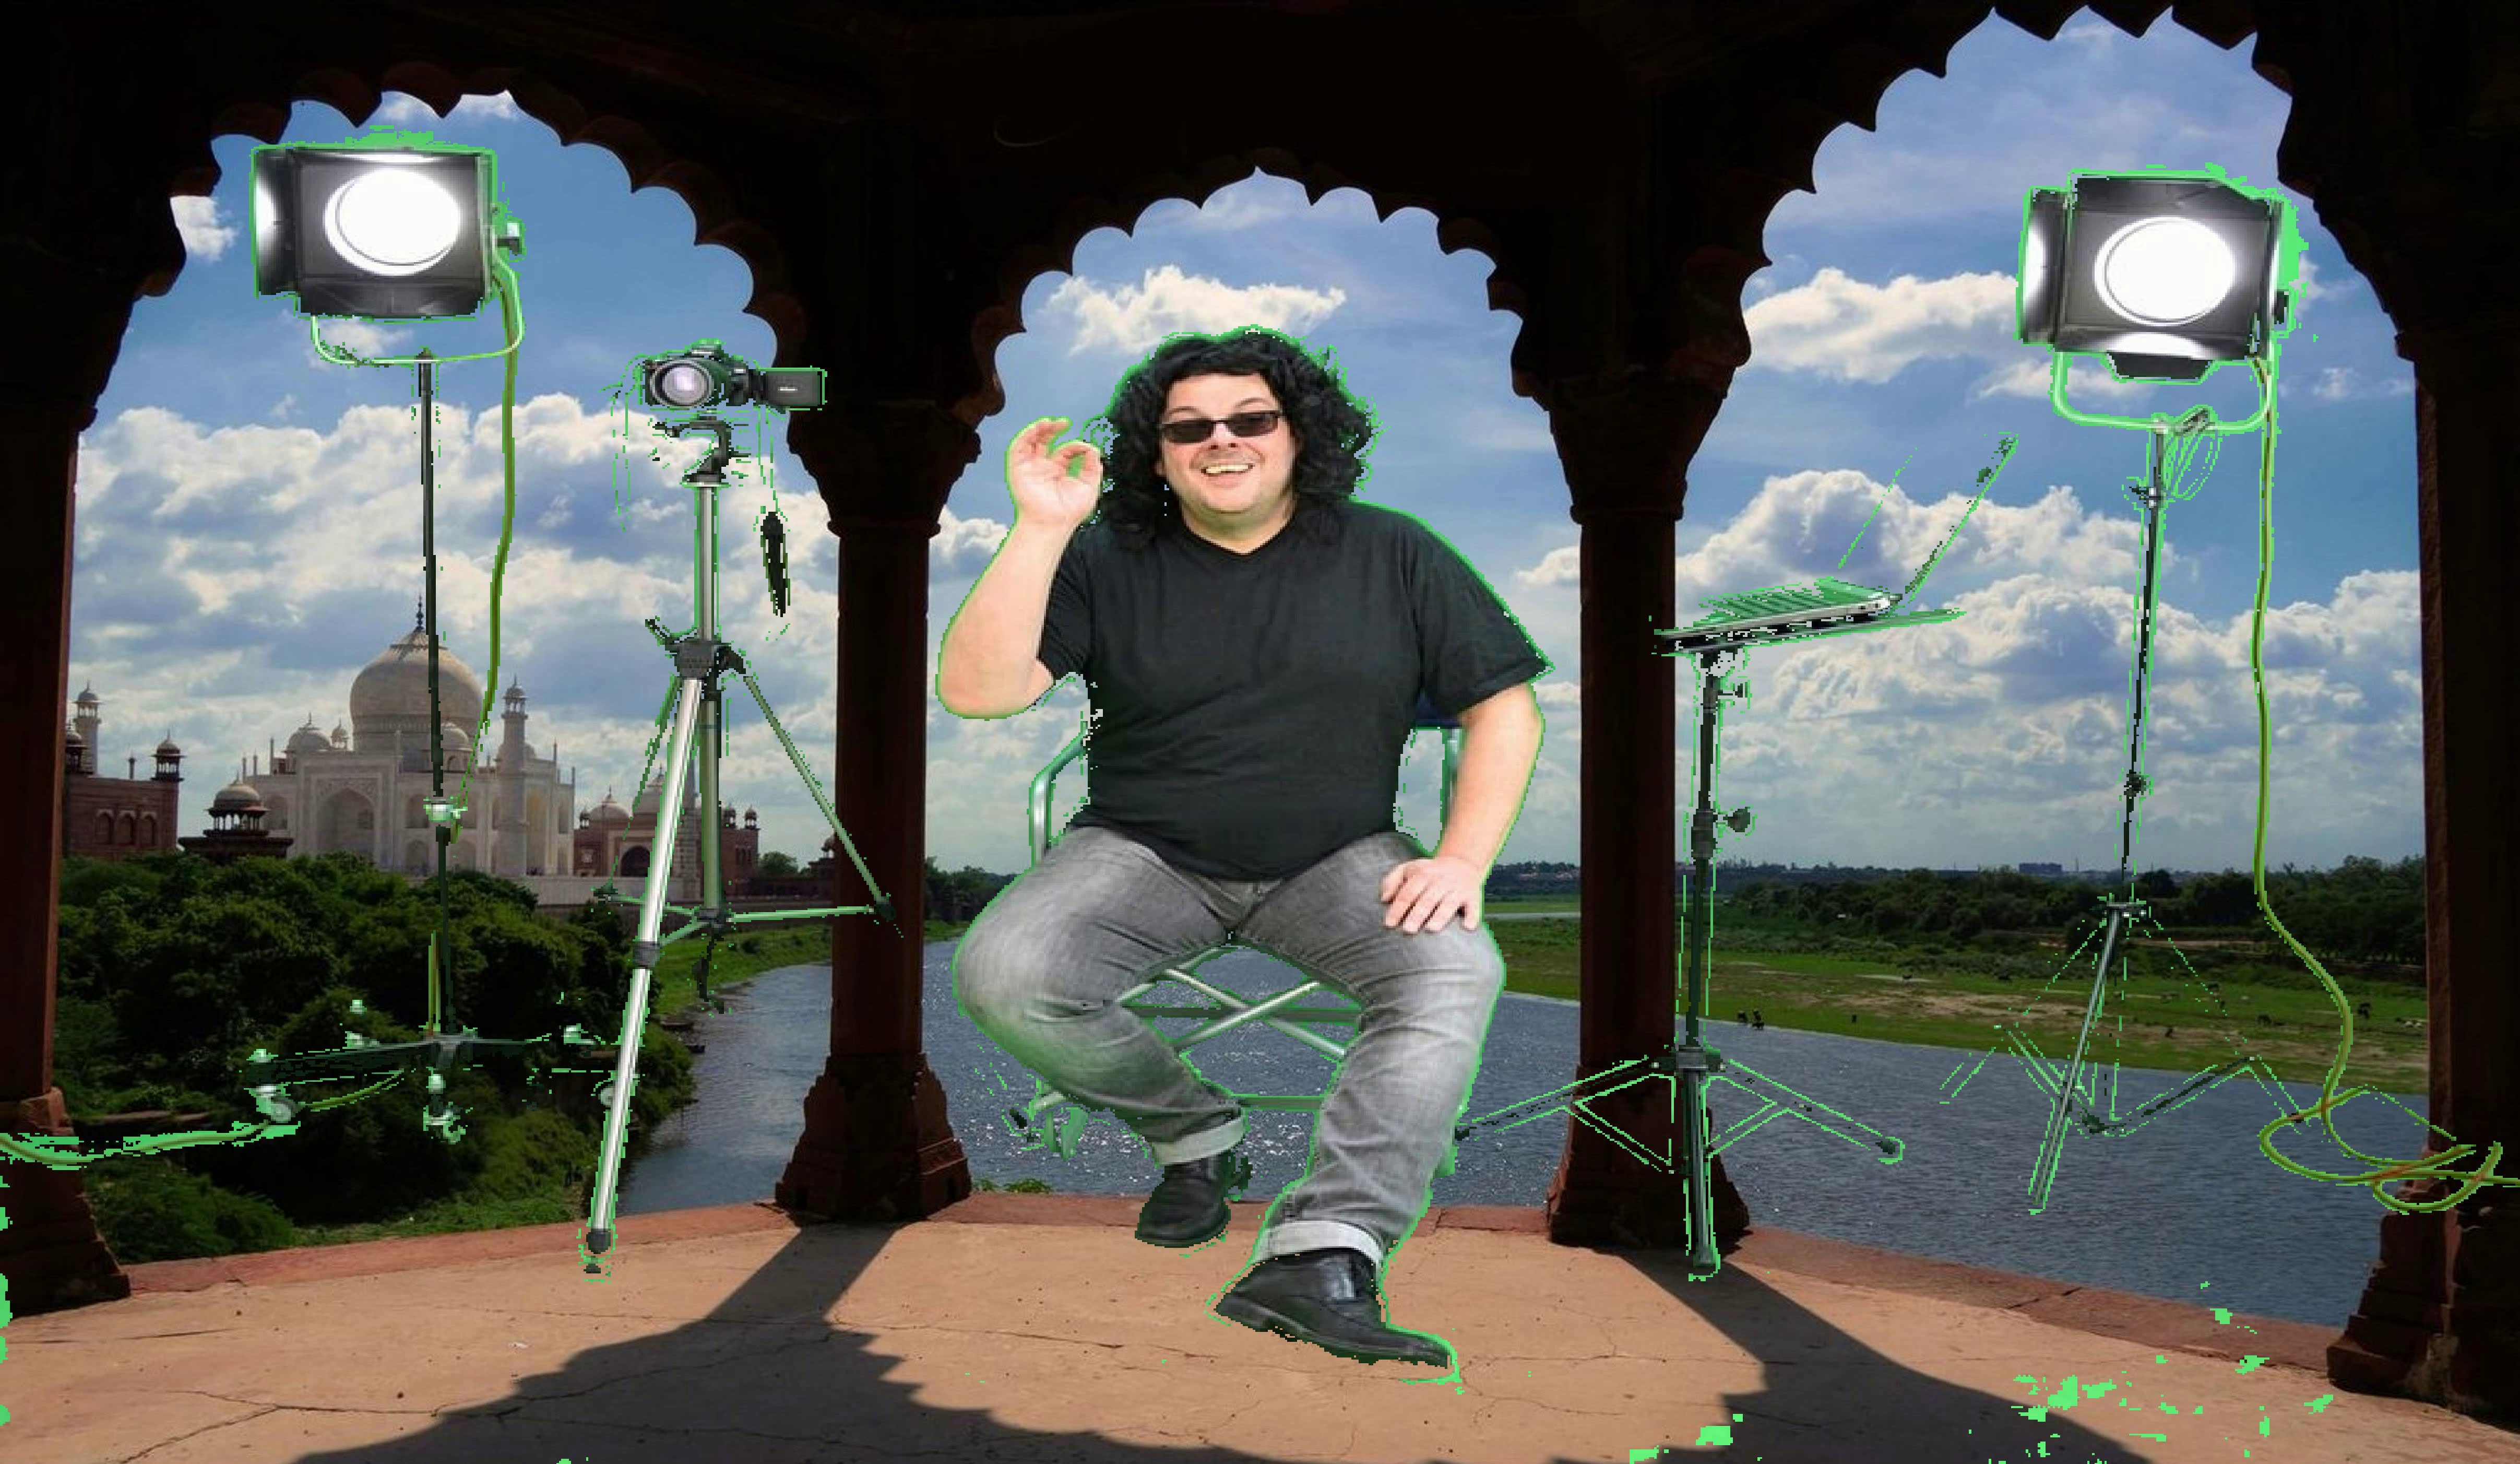
\includegraphics[width=\textwidth]{output/fade_transition_25.jpg}
        \caption{Last Frame}
    \end{subfigure}
    \hfill
    \caption{Fade transition on chroma keying.}
    \label{fig:transition}
\end{figure}

\end{document}
